\documentclass[10pt]{article}

%---------------------------------------------------------------------
\usepackage[a4paper, headsep=-4in,bindingoffset=0in,%
left=2.5cm,right=2.5cm,top=2.5cm,bottom=2.5cm,%
footskip=.25in]{geometry}
\newcommand{\textBF}[1]{%
    \pdfliteral direct {2 Tr 0.3 w} %the second factor is the boldness
     #1%
    \pdfliteral direct {0 Tr 0 w}%
}
\usepackage{multirow}
\usepackage{soul}

\def\Plus{\texttt{+}}
%\usepackage[english]{babel}   
\usepackage[utf8]{inputenc}  
\usepackage[font=scriptsize]{caption}
\usepackage{tabularx}
%\DeclareCaptionFont{6pt}{\fontsize{6pt}{6pt}\selectfont}
\captionsetup[figure]{font={stretch=1}}  
%\usepackage{sectsty}
\usepackage{subcaption}
\usepackage{wrapfig}
\usepackage{layout}
\usepackage{graphicx}
\usepackage{verbatim}
\usepackage{listings}
\usepackage{mathptmx}

\usepackage{booktabs}
\usepackage{etoolbox}


\usepackage{lmodern}
\usepackage[T1]{fontenc}
\usepackage[backend=biber,style=apa,sorting=none]{biblatex}
\addbibresource{paperpile.bib}
%\pagenumbering{gobble}
\pagenumbering{arabic}

\graphicspath{{figs/}}
\setlength{\topmargin}{-10pt}
%\renewcommand{\baselinestretch}{1.5}

\usepackage{indentfirst}
\setlength{\parindent}{1cm}
\usepackage[table]{xcolor}

\setlength{\headsep}{1pt}
%---------------------------------------------------------------------

\begin{document} 

\begin{center}
{\large \section*{Systematic comparison of imaging biomarkers of chronic stroke motor outcome }}
\end{center}

\begin{center}
Emily Olafson$^1$, Keith Jamison$^1$, Amy Kuceyeski$^1$
\end{center}

    1. \textmd{Department of Radiology, Weill Cornell Medical College, New York City, New York, USA, 10021} 

%---------------------------------------------------------------------


\section{Abstract}
Ischemic stroke is a major cause of physical impairment, and up to a third of stroke survivors have poor motor outcomes five years after the event. However, the ability to predict long-term deficits from acute clinical information remains a challenge. The location of the stroke in the brain can explain some of the variance in long-term outcomes, and incorporating information about lesion location can improve prediction models. Automated lesion segmentation methods can now be used, but it is unclear how to optimally use volumetric lesion data to predict chronic motor outcomes. Several lesion biomarkers have been related to stroke motor outcome, but it is unclear whether they can accurately predict chronic impairments across a range of lesion topographies. Models that incorporate damage to additional sensorimotor regions beyond the primary motor cortex have been shown to explain more variance in post-stroke outcome than models that only incorporate primary motor cortex CST damage. These models typically incorporate damage to premotor, supplementary motor, pre-supplementary motor, and somatosensory cortices. Few studies have assessed the performance of these models with cross-validation. This paper presents a comparison of the predictive accuracy of several imaging biomarkers of post-stroke motor impairment using the ENIGMA dataset, a multi-site stroke lesion database. The models are compared using out-of-sample performance, and the results show that data-driven features outperform theory-driven features. The data-driven features also outperform models trained on chronic subjects when applied to acute subjects. These results highlight the potential of data-driven feature selection in identifying lesion-deficit associations beyond current theory-driven biomarkers.

\section{Introduction}
Ischemic stroke is a leading cause of physical impairment worldwide. Up to one-third of stroke survivors have poor motor outcomes five years after stroke, but the ability to predict long-term deficits from acute clinical information is still a major challenge.

The location of the stroke in the brain explains some of the variance in long-term outcomes, and models of stroke outcome are improved by incorporating information about lesion location. Lesion segmentations, once requiring  delineation by experts, can now be performed with automated methods requiring minimal manual editing (\cite{Pustina2016-qu}). However, it is currently unclear how to optimally relate lesion data to chronic motor outcomes (\cite{Sperber2020-kp, Kasties2021-rm}), and to what extent lesion data can predict deficits in new patients.

The ultimate application of stroke lesion biomarkers is to predict future deficit scores for patients in whom only imaging, or other limited clinical data, is available. Doing so will require machine learning models whose parameters have been optimized through prior training on stroke datasets. Most lesion-based biomarkers have been related to motor deficits within a clinical sample, but few studies have assessed whether those models perform well on new data.

Several biomarkers of stroke motor outcomes have been derived from lesion data. The most widely-employed is the corticospinal tract (CST) lesion load, or the proportion of voxels in the ipsilesional corticospinal tract (typically originating from primary motor cortex) that intersect with the lesion (\cite{Zhu2010-qh, Feng2015-du}). This biomarker has been related to motor deficits in the acute phase of stroke, but it is unclear whether this biomarker can accurately predict chronic impairments across a wide range of lesion topographies (for review, see \cite{Kim2017-xe}). Models that incorporate information about how the lesion damages secondary sensorimotor regions, i.e. regions beyond the primary motor cortex that are still related to motor behavior, explain more variance in post-stroke outcome than models that incorporate information about primary motor cortex CST damage alone (\cite{Ito2022-em, Sperber2021-lw, Rondina2016-ds, Rondina2017-ij, Schulz2012-yy}). For instance, \cite{Ito2022-em} have shown that models that use lesion load of sensorimotor tracts, specifically tracts originating from the ventral premotor cortex, better predict stroke motor severity compared to models that only use M1-CST-LL. These more complex models tend to incorporate damage to premotor, supplementary motor, pre-supplementary motor, and somatosensory cortices (\cite{Ito2022-em,Schulz2012-yy, Sperber2021-lw, Rondina2016-ds, Rondina2017-ij}).

Variables that are significantly associated with outcomes (typically derived from an inference-based, hypothesis-testing framework), may not be the optimal set of variables to use in predictive models (\cite{Bzdok2020-py}). Indeed, the optimal set of features extracted from lesion data may not be directly related to hemiparesis per se (\cite{Sperber2021-lw}). Because of the hierarchical and non-random distribution of lesion topography (\cite{Mah2014-cb,Wang2019-dz}), damage to areas outside of the motor system may meaningfully predict chronic motor impairment (\cite{Sperber2021-lw}). Machine learning models that incorporate features in a data-driven way may be able to discover lesion-deficit associations beyond the current suite of theory-driven biomarkers like those in the motor system (\cite{Kasties2021-rm, Calesella2021-kp}). We estimated structural disconnection across all gray matter regions in the brain using the Network Modification tool (\cite{Kuceyeski2013-nk}) and used data-driven feature selection to identify regions that were relevant for predicting chronic motor outcomes. 



In this paper, we robustly compare the predictive accuracy of several imaging biomarkers of post-stroke motor impairment by assessing their out-of-sample performance using the ENIGMA dataset, a multi-site stroke lesion database (\cite{Liew2020-ps}). We compare theory-driven features (i.e. motor-related CST lesion load) with data-driven imaging features. 


\section{Materials and methods}
\subsection{Materials}
A subset of cross‐sectional data from the ENIGMA Stroke Recovery Working Group database (available as of 10 Sept. 2021) was used. Details of the ENIGMA Stroke Recovery procedures and methods are available in (\cite{Liew2020-ps}). The data were derived from 22 research studies (sites) (Table \ref{table:Demographics}). Informed consent was obtained from all subjects, and data were collected in compliance with each institution’s local ethical review boards and in accordance with the Declaration of Helsinki.

ENIGMA Stroke Recovery participants with the following data were included: (1) high‐resolution (1‐mm isotropic) T1‐weighted brain MRI (T1w) acquired with a 3T MRI scanner; (2) time since stroke at time of imaging greater than 180 days; (3) age, (4), sex, and (5) assessment of motor function (from one of several tests: FMA‐UE; acquired on a scale from 0 to 66: 0=severe sensorimotor impairment, 66=no sensorimotor impairment and normalized to the range 0 to 1 where 0=severe sensorimotor impairment), ARAT; NIHSS \hl{*In the process of obtaining more information from Lei/Bethany, ideally a breakdown of number of subjects for each test*}). 

Because we were interested in predicting chronic impairments, we only included participants with chronic stroke (defined as data acquired at least 180 days poststroke (\cite{Bernhardt2017-av}). Behavioral data were collected within approximately 72 hours of the MRI. 


Exclusion criteria included participants with no identifiable lesions. 

Inclusion criteria: subjects had to have a chronicity variable, normed motor score, and imaging.
For a subset of the models, subjects had to have age, sex, and days post stroke. A subset of subjects did not have data on their age, sex, and days post stroke (full sample N = 629, median normalized motor score = 0.7, IQR = 0.5) .
Lesions were segmented by the ENIGMA consortium and lesion masks were normalized to $1mm^3$ MNI v6 space. 

\begin{table}[h]
\centering
\caption{Site breakdown of total sample size (N), number of females (F) and males (M), and information about age (years), normed motor scores, and time since stroke (months). IQR, interquartile range}
\label{table:5}
\begin{tabular}{llllll}
\toprule
 & Total N. & Median age (y) & Median motor score & Median time since stroke  \\
Site ID & (F/M) & (IQR, min-max) & (IQR, min-max) &   (mos.) (IQR, min-max) \\
\midrule
r001 & 39 (10/29) & 61.0 (17.0, 31.0-80.0) & 0.65 (0.23, 0.00-0.88) & 23.5 (40.0, 6.7-178.2) \\
r002 & 12 (6/6) & 69.5 (11.5, 39.0-85.0) & 0.50 (0.41, 0.20-0.73) & 73.2 (51.9, 24.4-207.4) \\
r003 & 15 (6/9) & 61.0 (16.5, 33.0-85.0) & 0.24 (0.20, 0.08-0.61) & 48.8 (67.6, 6.1-205.4) \\
r004 & 19 (7/12) & 44.0 (14.5, 30.0-68.0) & 0.17 (0.16, 0.02-0.51) & 50.4 (81.9, 12.6-226.8) \\
r005 & 27 (12/15) & 66.0 (16.5, 44.0-81.0) & 0.79 (0.45, 0.12-0.98) & 31.4 (27.8, 7.4-150.1) \\
r009 & 60 (17/43) & 71.0 (7.2, 24.0-81.0) & 0.96 (0.12, 0.00-1.00) & 27.4 (9.3, 6.4-46.6) \\
r025 & 16 (3/13) & 64.5 (13.2, 38.0-88.0) & 0.98 (0.58, 0.00-1.00) & 14.2 (10.2, 6.1-66.1) \\
r027 & 28 (8/20) & 57.0 (10.2, 37.0-81.0) & 0.30 (0.16, 0.14-0.57) & 19.3 (24.7, 6.1-166.7) \\
r028 & 21 (6/15) & 63.0 (9.0, 23.0-75.0) & 0.82 (0.24, 0.35-1.00) & 26.5 (37.5, 6.7-114.5) \\
r031 & 1 (0/1) & 52.0 (0.0, 52.0-52.0) & 0.68 (0.00, 0.68-0.68) & 6.1 (0.0, 6.1-6.1) \\
r034 & 15 (6/9) & 58.4 (11.1, 32.4-80.0) & 0.82 (0.20, 0.58-0.95) & 61.3 (68.3, 11.8-141.6) \\
r035 & 15 (6/9) & 64.0 (18.0, 31.0-83.0) & 0.64 (0.52, 0.15-0.94) & 33.5 (22.9, 16.3-52.9) \\
r038 & 18 (7/11) & 67.0 (10.0, 30.0-83.0) & 1.00 (0.12, 0.35-1.00) & 15.1 (10.1, 6.4-30.9) \\
r040 & 14 (7/7) & 63.5 (9.8, 28.0-80.0) & 0.68 (0.47, 0.20-1.00) & 14.1 (17.5, 6.9-79.4) \\
r042 & 22 (11/11) & 48.5 (15.5, 25.0-76.0) & 0.64 (0.19, 0.39-0.80) & 29.6 (36.4, 6.1-207.5) \\
r044 & 4 (0/4) & 68.0 (9.2, 64.0-77.0) & 0.52 (0.25, 0.33-0.70) & 43.7 (52.9, 20.3-195.2) \\
r045 & 4 (1/3) & 62.0 (5.2, 50.0-65.0) & 0.49 (0.24, 0.20-0.74) & 96.1 (59.0, 60.0-189.1) \\
r046 & 11 (3/8) & 62.0 (10.5, 42.0-76.0) & 0.50 (0.29, 0.17-0.91) & 86.3 (83.4, 12.9-360.2) \\
r047 & 44 (14/30) & 65.5 (12.0, 43.0-93.0) & 0.65 (0.44, 0.06-0.98) & 38.1 (53.7, 6.0-171.6) \\
r048 & 43 (16/27) & 68.0 (12.5, 37.0-80.0) & 0.79 (0.44, 0.00-1.00) & 46.2 (49.8, 6.8-174.9) \\
r052 & 32 (12/20) & 63.0 (13.5, 34.0-85.0) & 0.41 (0.09, 0.21-0.52) & 39.1 (42.2, 6.1-247.1) \\
r053 & 2 (1/1) & 65.0 (3.0, 62.0-68.0) & 0.63 (0.25, 0.38-0.88) & 6.2 (0.1, 6.1-6.3) \\
\hline\\
All sites & 462 (159/303) & 63.1 (17.0, 23.0-93.0) & 0.7 (0.5, 0.0-1.0) & 31.3 (0.1, 6.0-360.2)  \\
\bottomrule
\end{tabular}
\end{table}




\subsection{Derivation of lesion biomarkers}
\subsubsection*{Lesion load of the ipsilesional primary motor cortex corticospinal tract}
The lesion load of the corticospinal tract originating from the primary motor cortex (M1-CST-LL) has been associated with motor impairment in several stroke studies. The M1-CST-LL was calculated as the proportion of lesioned voxels intersecting with a binarized ipsilesional M1-CST template (\cite{Zhu2010-qh}). Specifically, lesion load was calculated in 1mm MNIv6 space as:
\begin{equation}
    \textit{Lesion load} = \frac{\textit{Number of lesioned voxels intersecting with  tract}}{\textit{Number of voxels in tract}}
\end{equation}
Left and right hemisphere M1-CST segmentations in MNI space were obtained from the high-resolution sensorimotor area tract template (SMATT) (\cite{Archer2018-ti}). M1-CST Lesion load had a heavy tail distribution (Figure \ref{lesion_load_dist}a).
 
\subsubsection*{Lesion load of sensorimotor tracts}
Sensorimotor tract segmentations were obtained from the sensorimotor area tract template (SMATT), a set of 12 tracts derived from probabilistic tractography seeded in the left and right primary motor cortex (M1), dorsal and ventral premotor cortex (PMd and PMv, respectively), supplementary motor area (SMA), pre-supplementary motor area (pre-SMA), and primary somatosensory cortex (S1) (Figure \ref{fig:fig1}) (\cite{Archer2018-ti}). Lesion load was calculated as above, for all 12 tracts (i.e. across both hemispheres) and for 6 ipsilesional tracts. For subjects with brainstem, cerebellar, and/or bilateral cerebral strokes, ipsilesional lesion load was calculated as the average lesion load of the left and right hemisphere tracts.

Lesion loads from all tracts were positively correlated with one another and negatively correlated with motor scores (Figure \ref{lesion_load_dist}b,c, \ref{smatt_pairwise_correlations}, \ref{smatt_pairwise_correlations_bi}). 
%\subsubsection*{Deriving ChaCo scores (change in connectivity) from lesion masks}

\begin{figure}
\begin{subfigure}{1\textwidth}
  \centering
  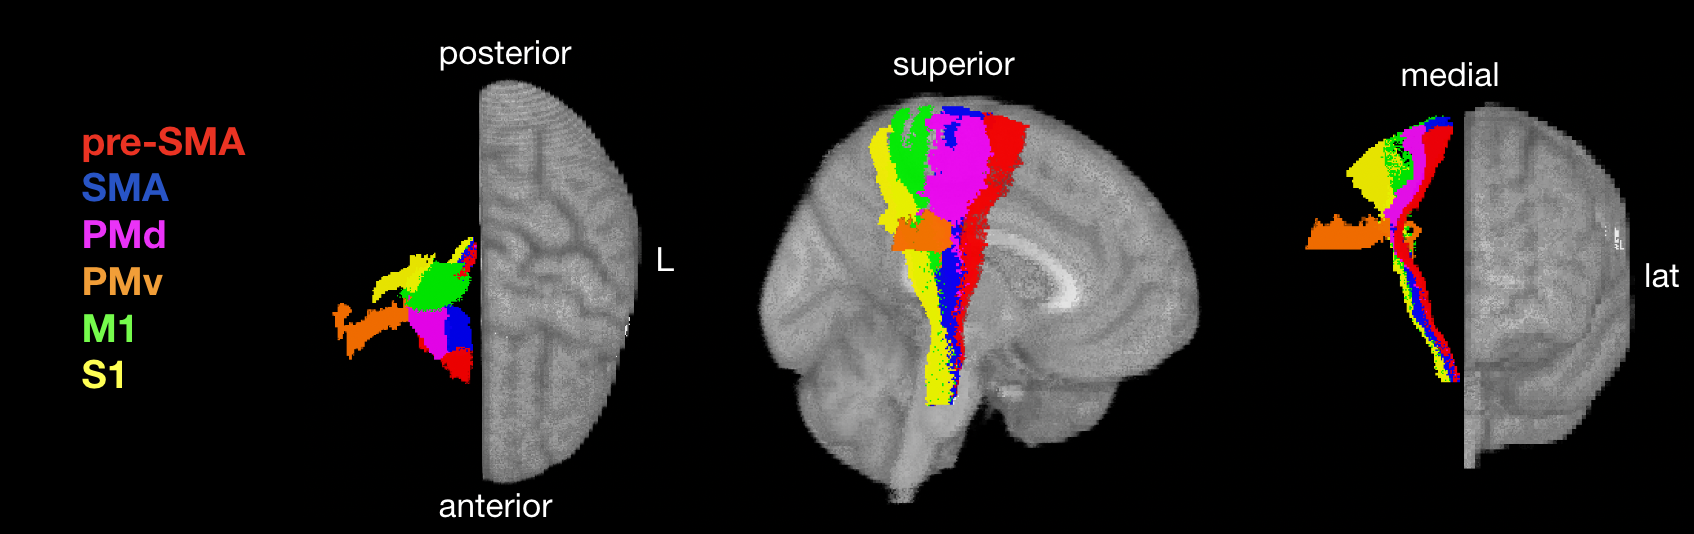
\includegraphics[width=1\linewidth]{figures/smatt_template.png}
  \caption{Sensorimotor tract template atlas (SMATT), displaying only right hemisphere tracts. Includes supplementary motor area (SMA), dorsal premotor cortex (PMd), ventral premotor cortex (PMv), pre-supplementary motor area (pre-SMA), primary sensory cortex (S1),  and primary motor cortex (M1)}
  \label{fig:fig1}
\end{subfigure}
\caption{Lesion biomarkers}
\label{fig:fig}

\begin{subfigure}{1\textwidth}
  \centering
  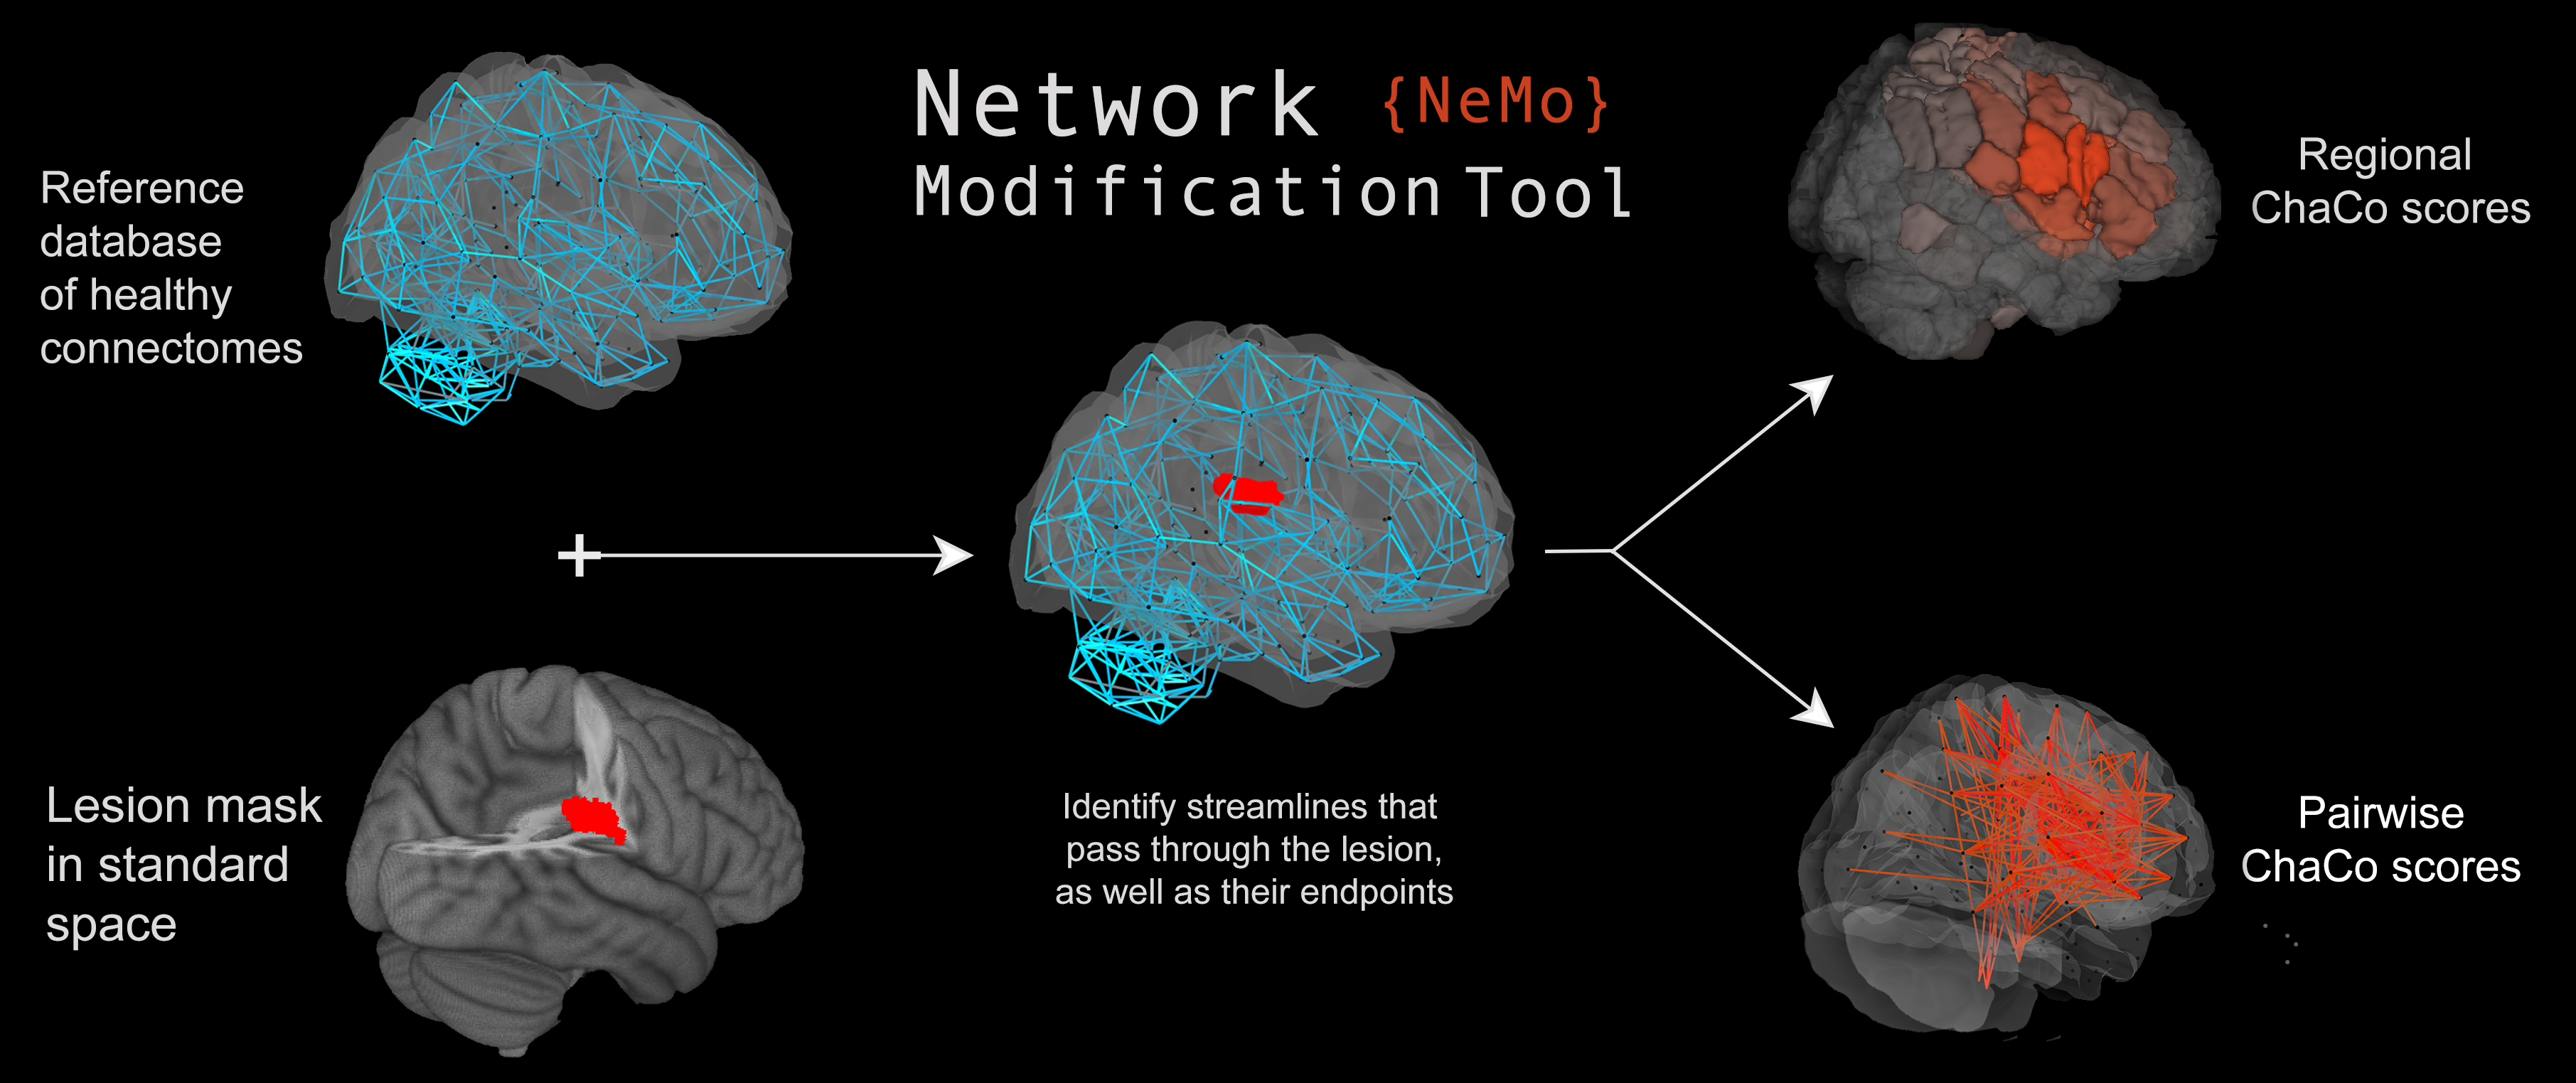
\includegraphics[width=1\linewidth]{figures/NetworkModificationTool.png}
  \caption{Overview of the Network Modification tool. Binary lesion masks in MNI space representing the presence of a stroke lesion in a given voxel are provided by the user. Each lesion mask is embedded into 420 unrelated healthy structural connectomes (separately for each healthy subject) and the regional or pairwise change in connectivity (ChaCo) scores are calculated and averaged across healthy subjects. }
  \label{fig:fig2}
\end{subfigure}

\end{figure}

\subsubsection*{Regional structural disconnection: ChaCo scores}

Lesion masks in $1mm^3$ MNI v6 space were processed with the Network Modification Tool (NeMo Tool) v2 pipeline (\cite{Kuceyeski2013-nk}) (https://github.com/kjamison/nemo for more detailed information). Given a lesion mask, the NeMo tool produces outputs that reflect the impact of the lesion on the white matter tracts connecting brain regions. The NeMo tool identifies every white matter streamline that intersects with a lesion and determines the brain regions at the endpoints of those streamlines, whose structural connections are putatively disrupted (Figure \ref{fig:fig2}). The NeMo tool uses a reference structural connectome dataset of 420 unrelated subjects from the Human Connectome Project (HCP) Young Adult database. Structural connectivity for HCP subjects was obtained using deterministic tractography (SD stream) with dynamic seeding, with additional SIFT2 weighting for each of 5 million streamlines (\cite{Smith2015-eb}). Regional change in connectivity (ChaCo) scores, or the ratio of the number of disrupted streamlines divided by the total number of streamlines for each region, were calculated for all grey matter regions. Regional ChaCo scores from two different altases were compared: the 86-region Desikan-Killiany Atlas (68 cortical regions $\Plus$ 18 subcortical regions, excluding brainstem) from FreeSurfer ("fs86" for short), which contains coarse anatomically parcellated regions (\cite{Desikan2006-vf,Fischl2002-lb}), and the 268-region Shen atlas ("shen268" for short), which contains more fine-grained functionally parcellated cortical and subcortical regions (\cite{Shen2013-zn}).


\subsection{Prediction models}
\subsubsection*{General framework}

Models were trained and evaluated using a 5-fold nested cross-validation loop. Data was first split into 5 training and tests folds, using an 80/20 train/test split. The size of each train/test fold is approximately 370/92 subjects, respectively. 

\subsubsection*{M1-CST-LL models}

\subsubsection*{Sensorimotor tract LL models}
Ridge regression was used to account for multicollinearity of imaging features. Lesion load values were normalized (by subtracting the mean across subjects and dividing by the l2-norm) prior to model fitting.

\subsubsection*{ChaCo models}

Ridge regression models were trained and evaluated using a 5-fold nested cross-validation loop. In the outer loop, the data was split into training and test partitions. Training data was further partitioned into training and validation in the inner loop. In the inner loop, two hyperparameters were optimized: the amount of regularization on regression coefficients ($\lambda$) and the number of features to include ($\kappa$). The correlation between all features (i.e. regional ChaCo scores) and motor scores was calculated and the features were ranked by absolute value correlation. The top $\kappa$ features were then included in the model. Importantly, feature selection was performed on the training/validation data after data was split into training and test sets, such that no hold-out test data was used in the selection of the set of features (\cite{Hastie2001-or}). The $\kappa$ values searched for FS86 spanned 30 values from 5 to 86, in log base-2 steps; the $\kappa$ values searched for shen268 spanned 30 values from 5 to 268, in log base-2 steps. 

Out of sample cross-validation schemes.

Because inference and prediction are different goals and the feature maps derived from both types of studies can vary widely (\cite{Sperber2021-lw, Bzdok2020-py}), we included a correlation-based feature selection step. 


\subsubsection*{Ensemble models}
In order to improve prediction accuracies, we evaluated whether performance would be improved by averaging predictions from multiple models, combining several imaging biomarker metrics alongside demographic features like age, sex, and days post stroke. A standard linear regression model was used to model the relationship between demographic information and motor impairment. 


\begin{itemize}
\item H1: Models including demographic information (age, sex, and days post stroke) alongside lesion data will perform better than models with lesion data or demographic data alone (i.e., variance explained from lesion data and demographic data is not redundant).
\item H2: Models including both lesion load and ChaCo scores will perform better than models with lesion load or ChaCo scores alone.
\end{itemize}

 The number of subjects in each train/test fold for models incorporating demographic information is approximately 370/92, respectively.

from the lesion load models and from the data-driven feature selection ChaCo models. These ensemble models were generated by training ChaCo-models and lesion load models separately, on the same subjects and with the same training/test/validation splits, and averaging the final predicted scores for each subject. 



\subsubsection*{Model performance}
Model performance was assessed by comparing true motor scores ($y$) with predicted scores ($\hat{y}$). Performance was calculated with Pearson's correlation coefficient, 
\begin{equation}
    r(y, \hat{y}) = \sqrt{\frac{\sum_i{\hat{y}-\bar{\hat{y}}}}{\sum_i{y-\bar{y}}}}
\end{equation}
where $\bar{y}$ is the mean of true motor scores and  $\bar{\hat{y}}$ is the mean of the predicted scores, and by the coefficient of determination, or $R^2$, which captures the percent of variation in motor scores explained by variation in the model predictors:
\begin{equation}
    R^2(y, \hat{y}) = 1 - \frac{Var(y-\hat{y})}{Var(y)}
\end{equation}


\subsubsection*{Code availability}
All analysis scripts that generated the results of the present study are readily accessible and open for reuse, with any stroke outcome score specified (https://github.com/emilyolafson/enigma$\_$predictions).


\section{Results}
\subsection*{Subject demographics}



Ridge regression models fit using the lesion load of left and right sensorimotor tracts best predicted chronic motor scores for new subjects, with an average correlation between true and predicted scores of 0.44 $\pm 0.01$ ($R^2 = 0.17$) (Figure \ref{analysis1}), performing significantly better than linear models fit with ipsilesional M1 corticospinal tract lesion load (average correlation = 0.40 $\pm ?$), ridge regression models with ipsilesional sensorimotor tract lesion load, and ridge regression models with data-driven selection of regional ChaCo scores.

All twelve sensorimotor tracts had significant (?) regression coefficients, suggesting that chronic motor scores are best predicted by a linear combination of lesion load to left and right hemisphere sensorimotor tracts. 
\\
\\
\begin{table}[h]
\centering
\caption{Test performance of all models evaluated, displaying median $R^2$ and median correlation of average hold-out performances (i.e. average across 5 outer folds) across 100 permutations. The first 5 rows contain results from models using lesion information only. The second 5 rows contain results from ensemble models that average predictions from lesion information and demographcis (age, sex, days post stroke). The final 6 rows contain results from ensemble models averaging predictions between two types of lesion information (lesion load predictions and ChaCo score predictions), with the final 3 rows showing results from ensemble models using lesion load, ChaCo scores, and demographics. Demog. = demographics, Ipsi. SMATT LL = ipsilesional sensorimotor tract template lesion load, L/R SMATT LL = left and right sensorimotor tract template lesion load, M1 CST LL = M1 corticospinal tract lesion load, ChaCo = Change in Connectivity, fs86 = FreeSurfer 86-region atlas}
\label{table:5}
\begin{tabular}{rrrrr}
\toprule
 &  & \multicolumn{2}{c}{Median performance} \\
 &  & Corr. (Std. dev.) & $R^2$ (Std. dev.) \\
\midrule
\multirow[t]{5}{*}{none} & M1 CST LL & 0.394 (0.006) & 0.152 (0.005) \\
 & Ipsi. SMATT LL & 0.435 (0.007) & 0.185 (0.007) \\
 & L/R SMATT LL & 0.439 (0.009) & 0.187 (0.009) \\
 & ChaCo (shen268) & 0.431 (0.016) & 0.181 (0.027) \\
 & ChaCo (fs86) & 0.429 (0.014) & 0.179 (0.013) \\
\multirow[t]{5}{*}{demog} & M1 CST LL $\Plus$ demog. & 0.436 (0.007) & 0.165 (0.005) \\
 & Ipsi. SMATT LL $\Plus$ demog. & 0.459 (0.006) & 0.186 (0.005) \\
 & L/R SMATT LL $\Plus$ demog. & 0.465 (0.009) & 0.189 (0.006) \\
 & ChaCo (shen268) $\Plus$ demog. & 0.457 (0.011) & 0.187 (0.010) \\
 & ChaCo (fs86) $\Plus$ demog. & 0.453 (0.010) & 0.181 (0.007) \\
\multirow[t]{6}{*}{chaco ll} & M1 CST LL $\Plus$ ChaCo (fs86) & 0.454 (0.008) & 0.197 (0.007) \\
 & Ipsi. SMATT LL $\Plus$ ChaCo (fs86) & 0.463 (0.009) & 0.206 (0.007) \\
 & L/R SMATT LL $\Plus$ ChaCo (fs86) & 0.463 (0.010) & 0.207 (0.009) \\
 & M1 CST LL $\Plus$ ChaCo (shen268) & 0.454 (0.008) & 0.197 (0.006) \\
 & Ipsi. SMATT LL $\Plus$ ChaCo (shen268) & 0.464 (0.009) & 0.208 (0.007) \\
 & L/R SMATT LL $\Plus$ ChaCo (shen268) & 0.463 (0.009) & 0.208 (0.007) \\
\multirow[t]{6}{*}{chaco ll demog} & M1 CST LL $\Plus$ ChaCo  (fs86) & 0.478 (0.007) & 0.196 (0.005) \\
 & Ipsi. SMATT LL $\Plus$ ChaCo  (fs86) & 0.483 (0.008) & 0.206 (0.006) \\
 & L/R SMATT LL $\Plus$ ChaCo  (fs86) & 0.485 (0.008) & 0.207 (0.006) \\
 & M1 CST LL $\Plus$ ChaCo  (shen268) & 0.478 (0.008) & 0.199 (0.005) \\
 & Ipsi. SMATT LL $\Plus$ ChaCo  (shen268) & 0.484 (0.010) & 0.208 (0.007) \\
 & L/R SMATT LL $\Plus$ ChaCo  (shen268) & 0.484 (0.010) & 0.208 (0.007) \\
\bottomrule
\end{tabular}
\end{table}


\begin{figure}[htp]
\centering
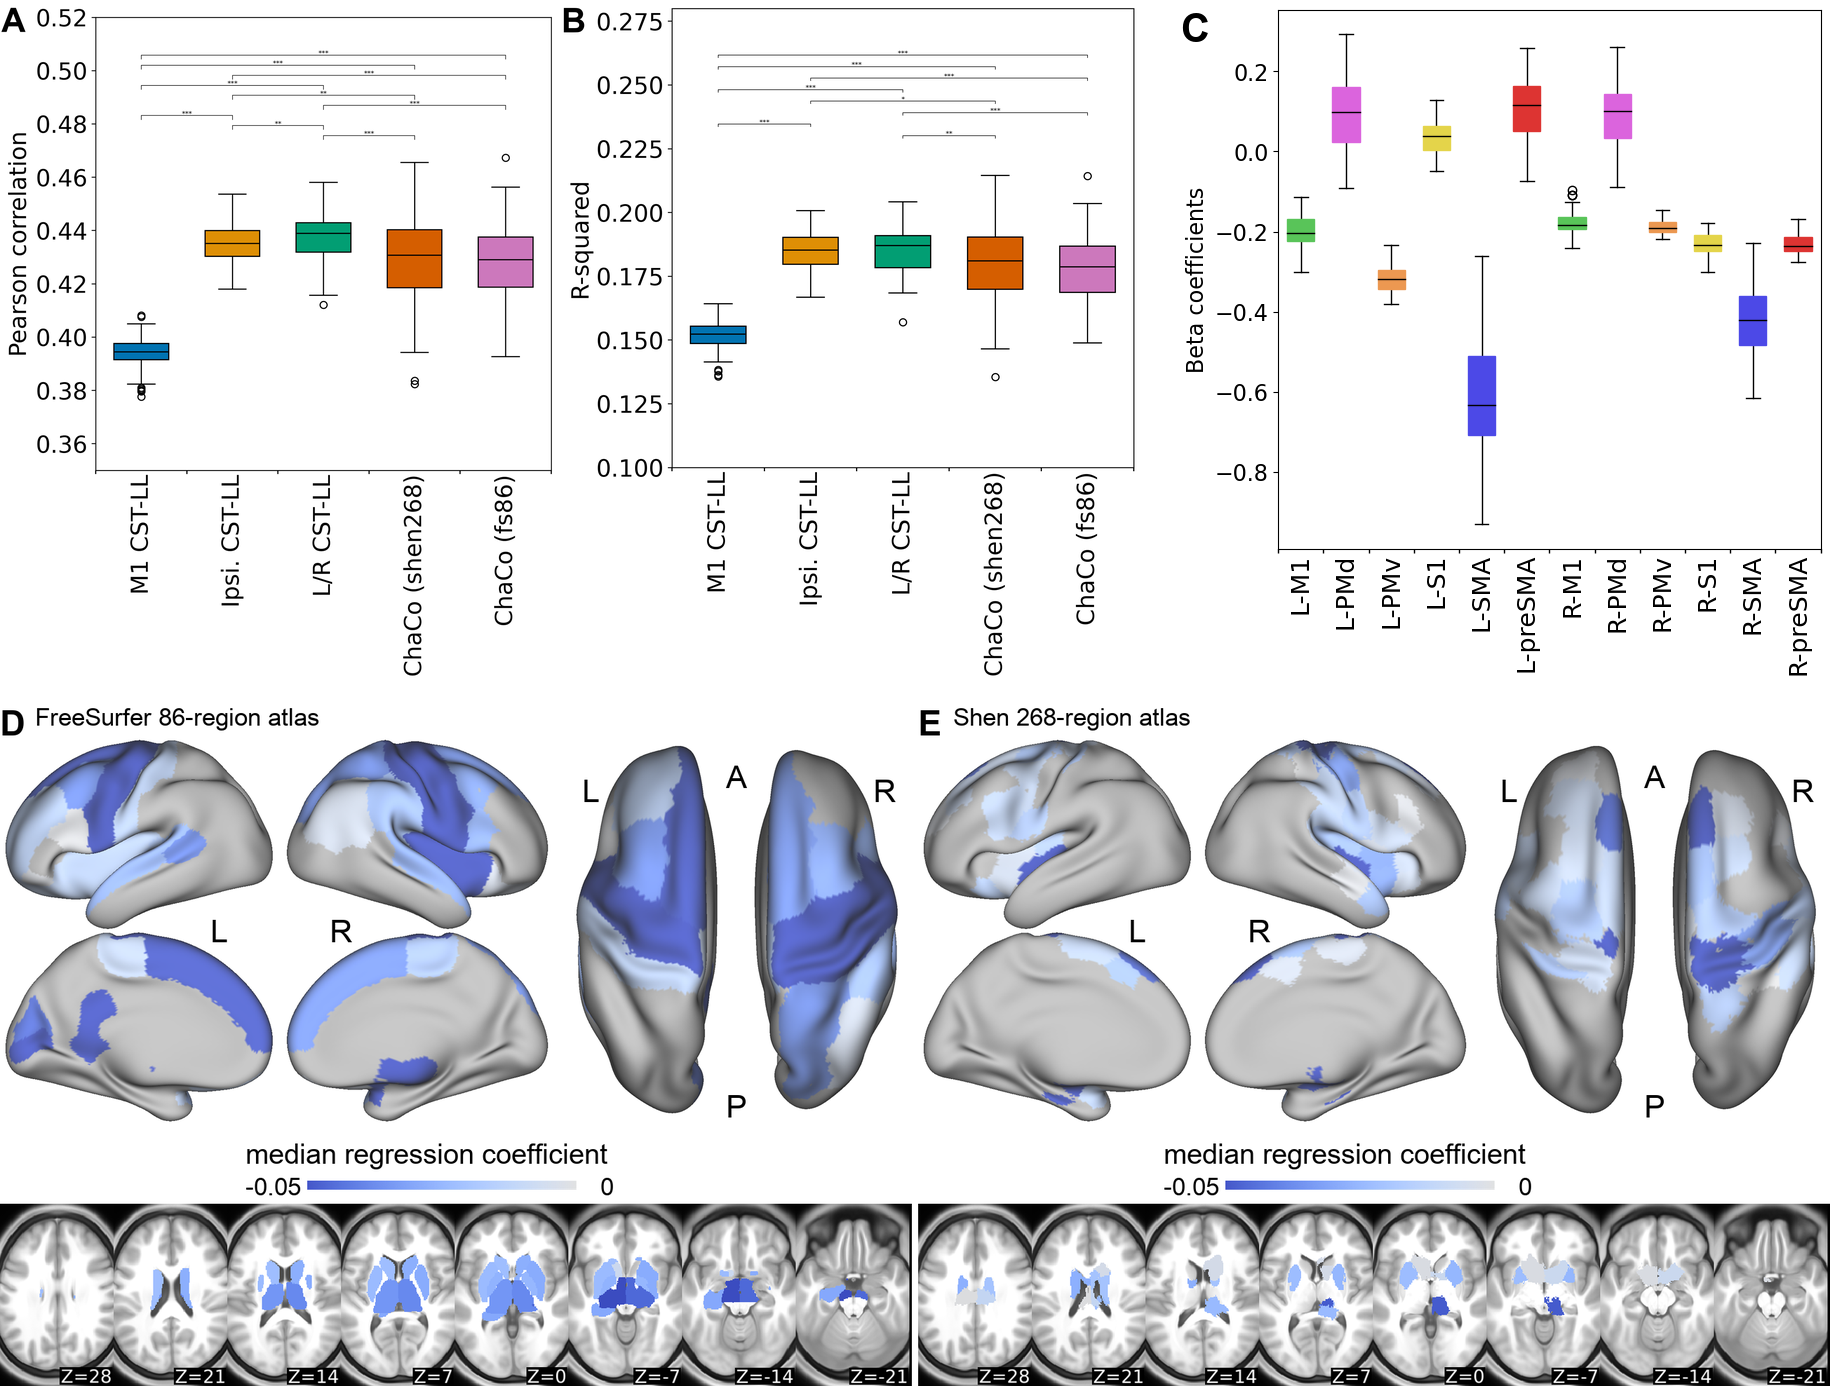
\includegraphics[width=1\linewidth]{figures/Analysis1.png}
\caption{Regression coefficients and model performance using standard KFold cross-validation (train/test splits shuffled). \textbf{A.} and \textbf{B.} display model performance (mean Pearson correlation/$R^2$ across 5 outer folds for 100 permutations of the data). Boxplots are colored abritrarily for clarify, where the box extends from the lower to upper quartile values of the data, with a line at the median. Whiskers represent the range of the data from [Q1-1.5*IQR, Q3+1.5*IQR].
Average feature weights for regions that were selected in at least half of the models (i.e., were included in the model in at least 250/500 outer folds). \textbf{C.} Sensorimotor area tract template feature importance for analysis 1. Includes primary motor cortex (M1), dorsal premotor cortex (PMd), ventral premotor cortex (PMv), supplementary motor area (SMA), pre-supplementary motor area (pre-SMA), primary sensory cortex (S1).}
\label{analysis1}
\end{figure}

\begin{figure}[htp]
\centering
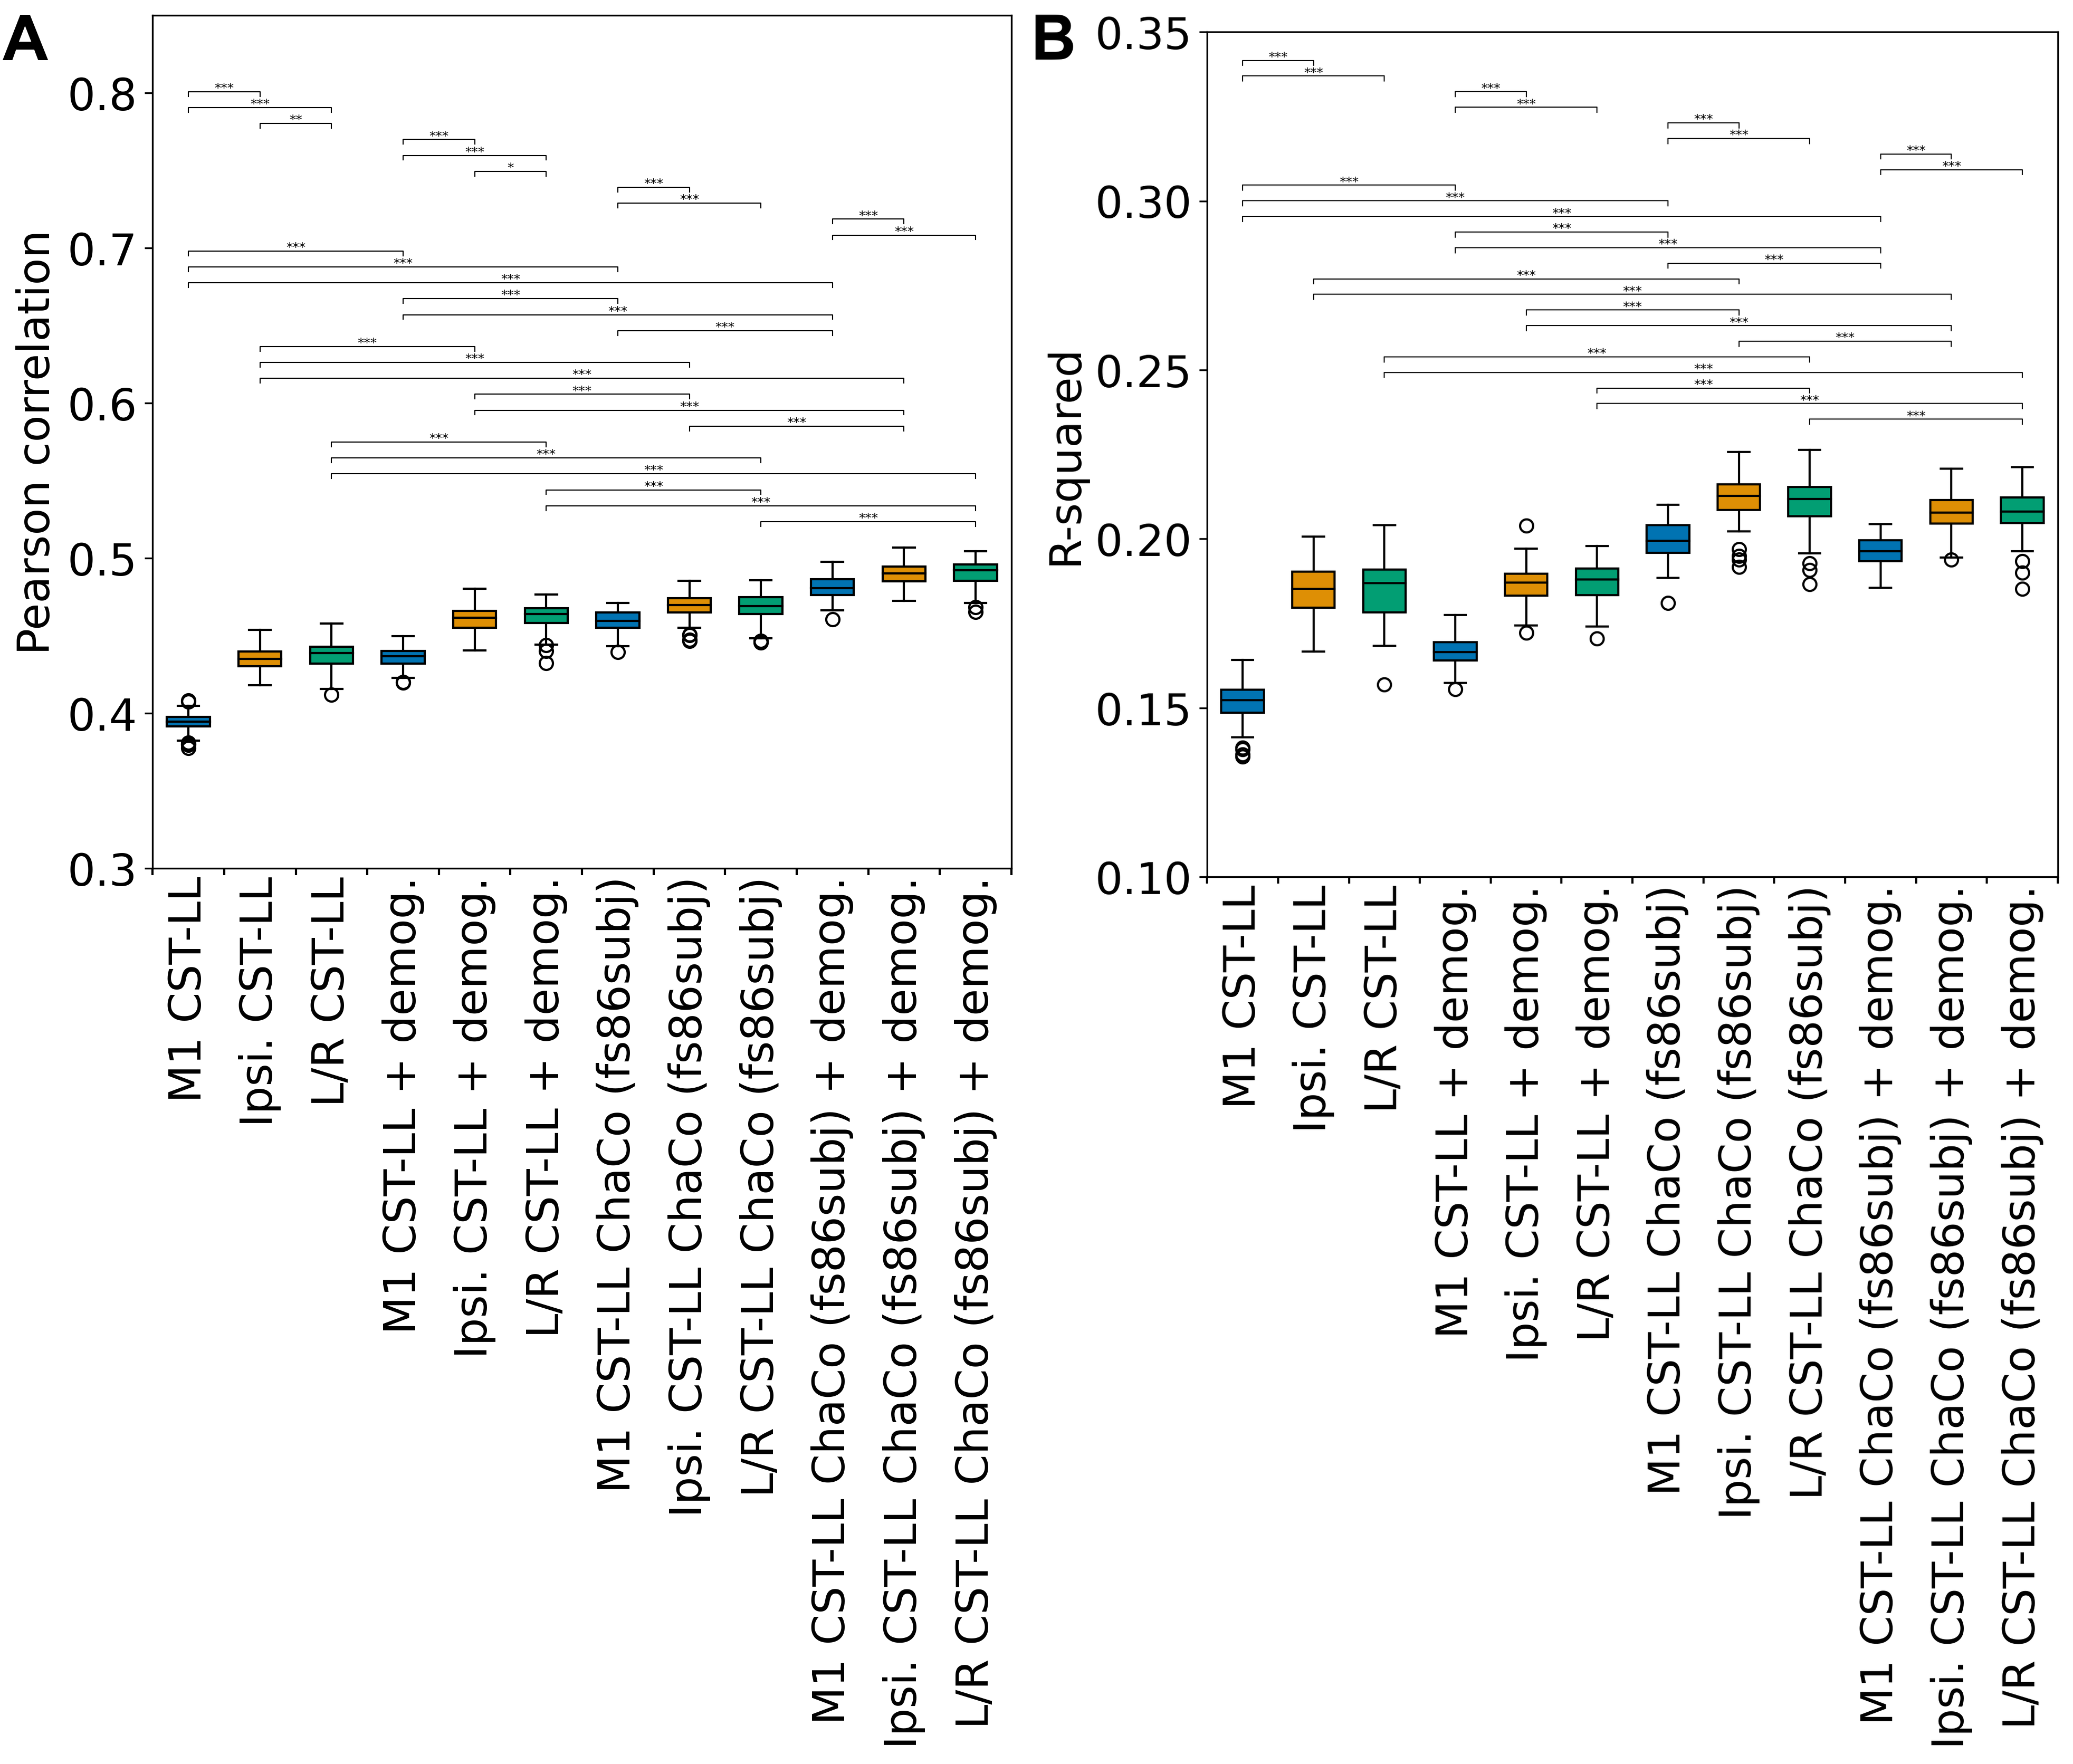
\includegraphics[width=1\linewidth]{figures/Analysis2.png}
\caption{Regression coefficients and model performance using Group KFold cross-validation (test/validate on independent imaging site). \textbf{A.} and \textbf{B.} display regression coefficients for regional ChaCo scores (FreeSurfer 86-region atlas, and Shen268-region atlas, respectively). Average feature weights for regions that were selected in at least half of the models (i.e., were included in the model in at least 250/500 outer folds). \textbf{C.} Sensorimotor area tract template feature importance for analysis 2. Includes primary motor cortex (M1), dorsal premotor cortex (PMd), ventral premotor cortex (PMv), supplementary motor area (SMA), pre-supplementary motor area (pre-SMA), primary sensory cortex (S1).}
\label{nemotool}
\end{figure}


\begin{figure}[htp]
\centering
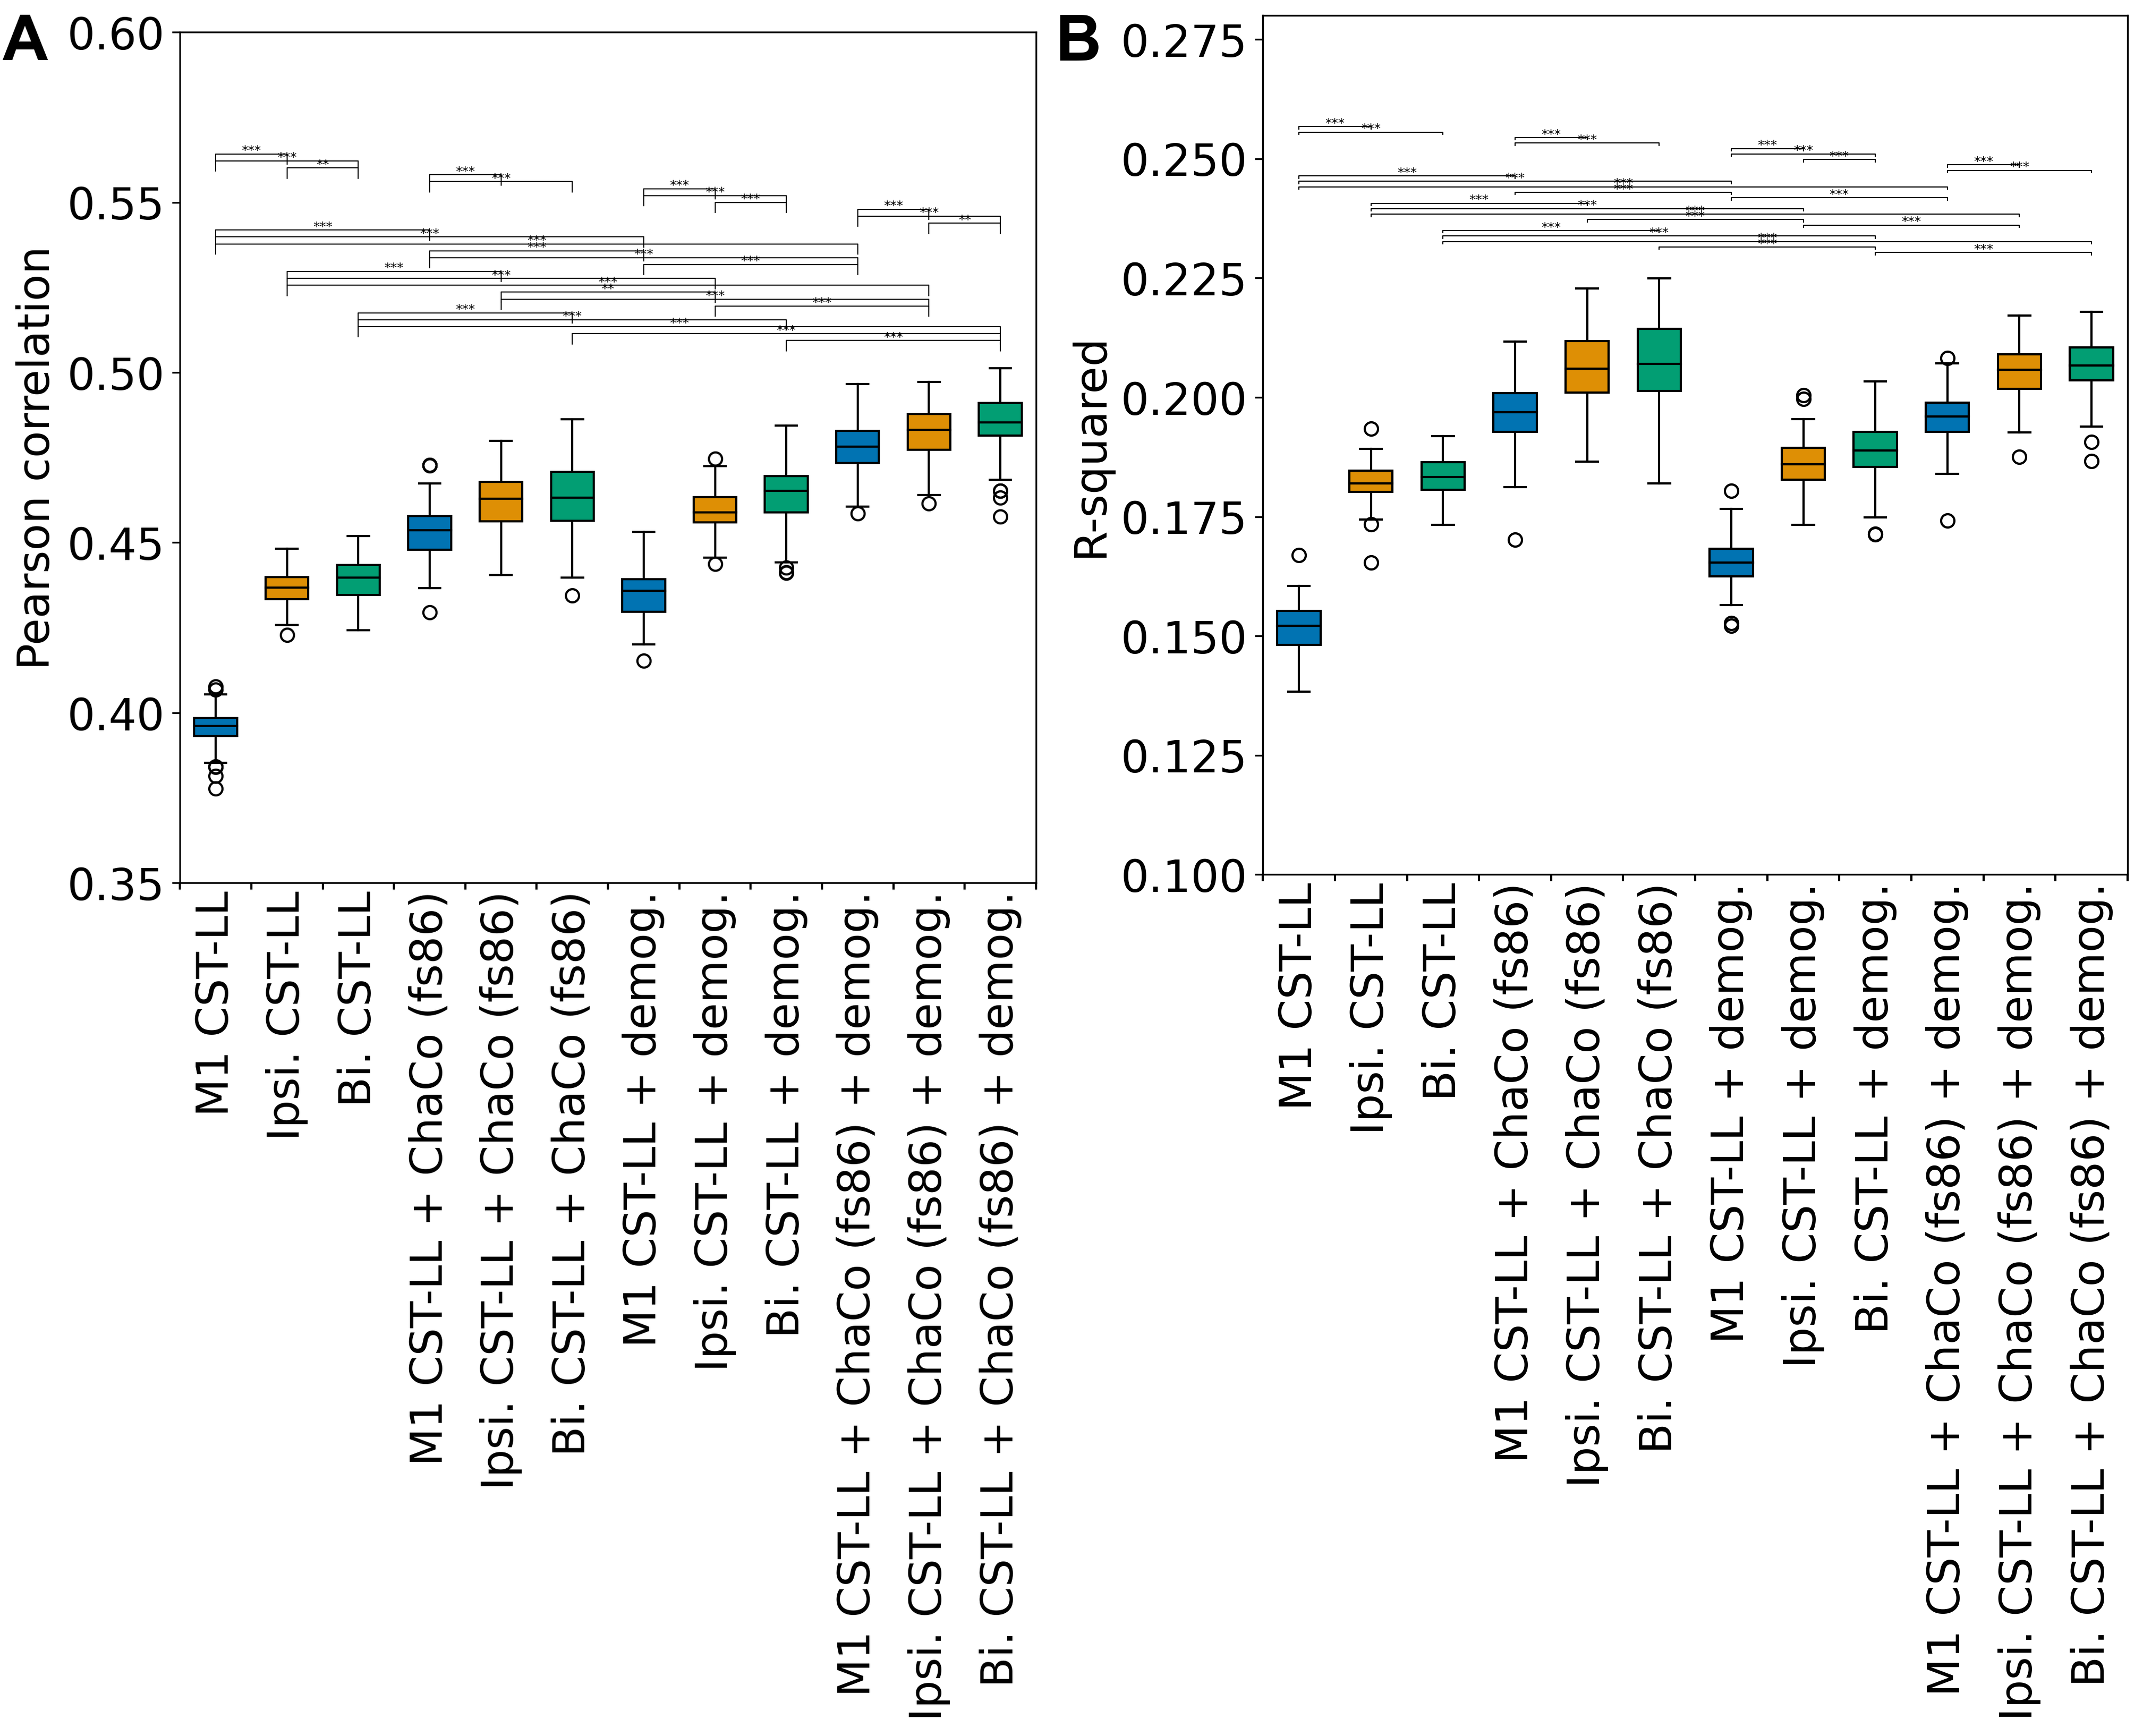
\includegraphics[width=1\linewidth]{figures/Analysis8.png}
\caption{Demographic ensemble model results. coefficients and model performance using Group KFold cross-validation (test/validate on independent imaging site). \textbf{A.} and \textbf{B.} display regression coefficients for regional ChaCo scores (FreeSurfer 86-region atlas, and Shen268-region atlas, respectively). Average feature weights for regions that were selected in at least half of the models (i.e., were included in the model in at least 250/500 outer folds). \textbf{C.} Sensorimotor area tract template feature importance for analysis 2. Includes primary motor cortex (M1), dorsal premotor cortex (PMd), ventral premotor cortex (PMv), supplementary motor area (SMA), pre-supplementary motor area (pre-SMA), primary sensory cortex (S1).}
\label{nemotool}
\end{figure}


\section{Discussion}

\clearpage

\newcommand{\beginsupplement}{%
\setcounter{table}{0}
\renewcommand{\thetable}{S\arabic{table}}%
\setcounter{figure}{0}
\renewcommand{\thefigure}{S\arabic{figure}}%
}

\printbibliography

\beginsupplement
\section*{Supplementary Figures}
\begin{figure}
\begin{subfigure}{0.5\textwidth}
  \centering
  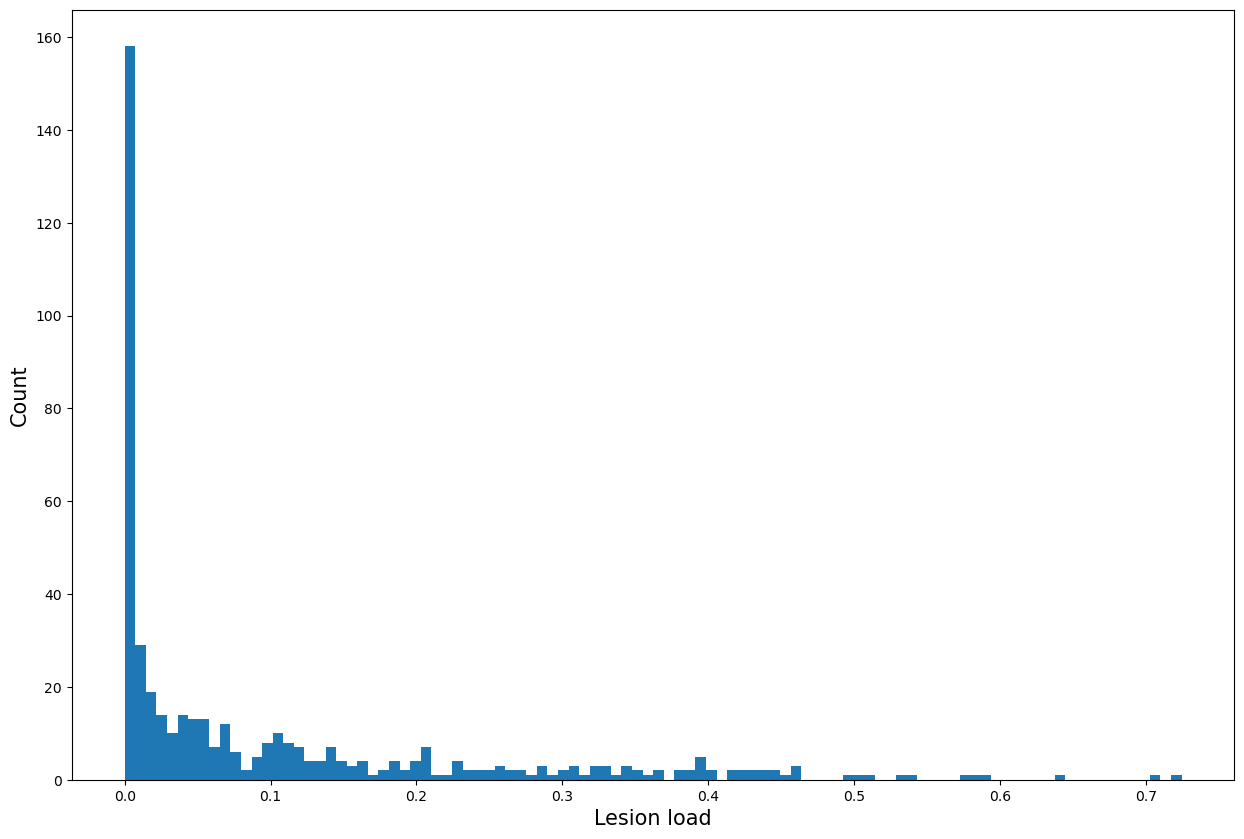
\includegraphics[width=1\linewidth]{figures/m1_lesionload.png}
  \caption{Distribution of M1-CST lesion load.}
  \label{fig:sfig1}
\end{subfigure}
\begin{subfigure}{0.5\textwidth}
  \centering
  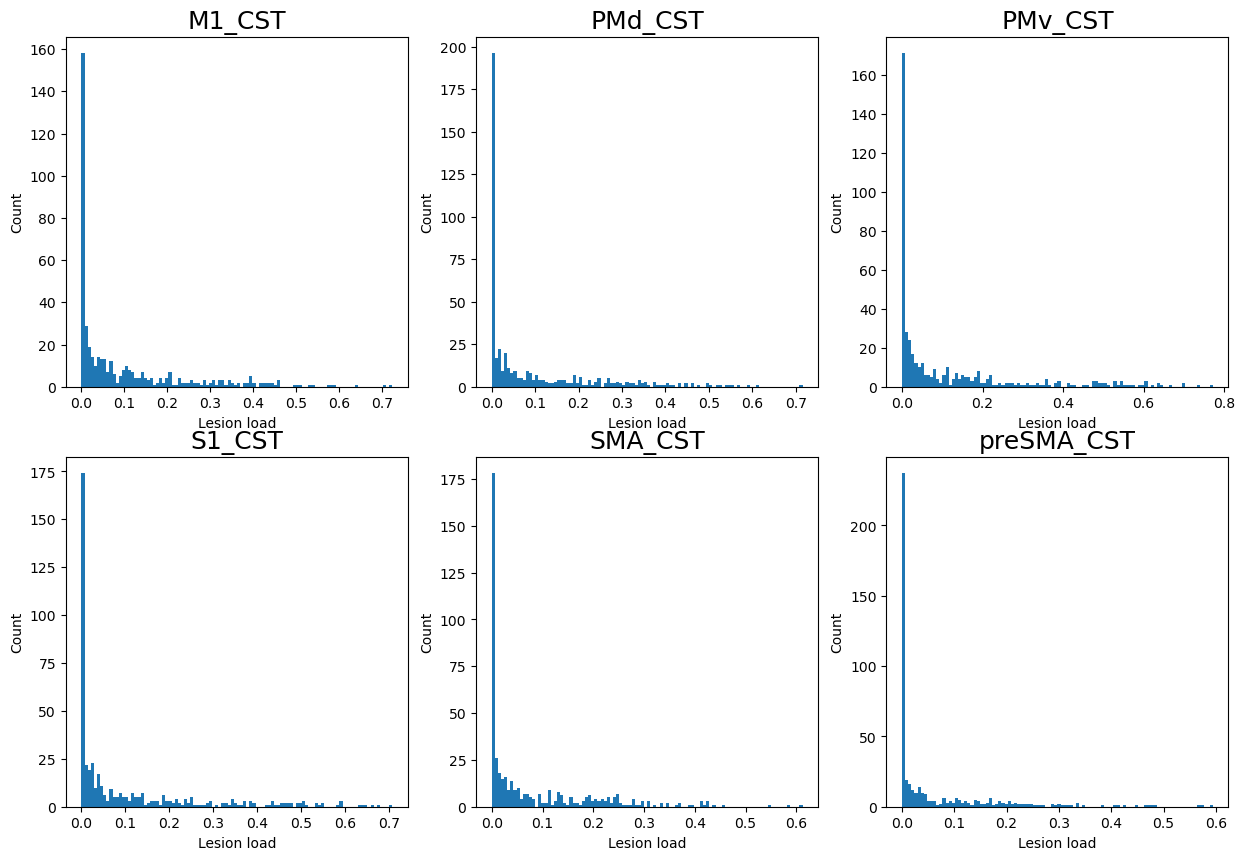
\includegraphics[width=1\linewidth]{figures/all_lesionload.png}
  \caption{Distributions of ipsilesional SMATT lesion load.}
  \label{fig:sfig2}
\end{subfigure}
\begin{subfigure}{1\textwidth}
  \centering
  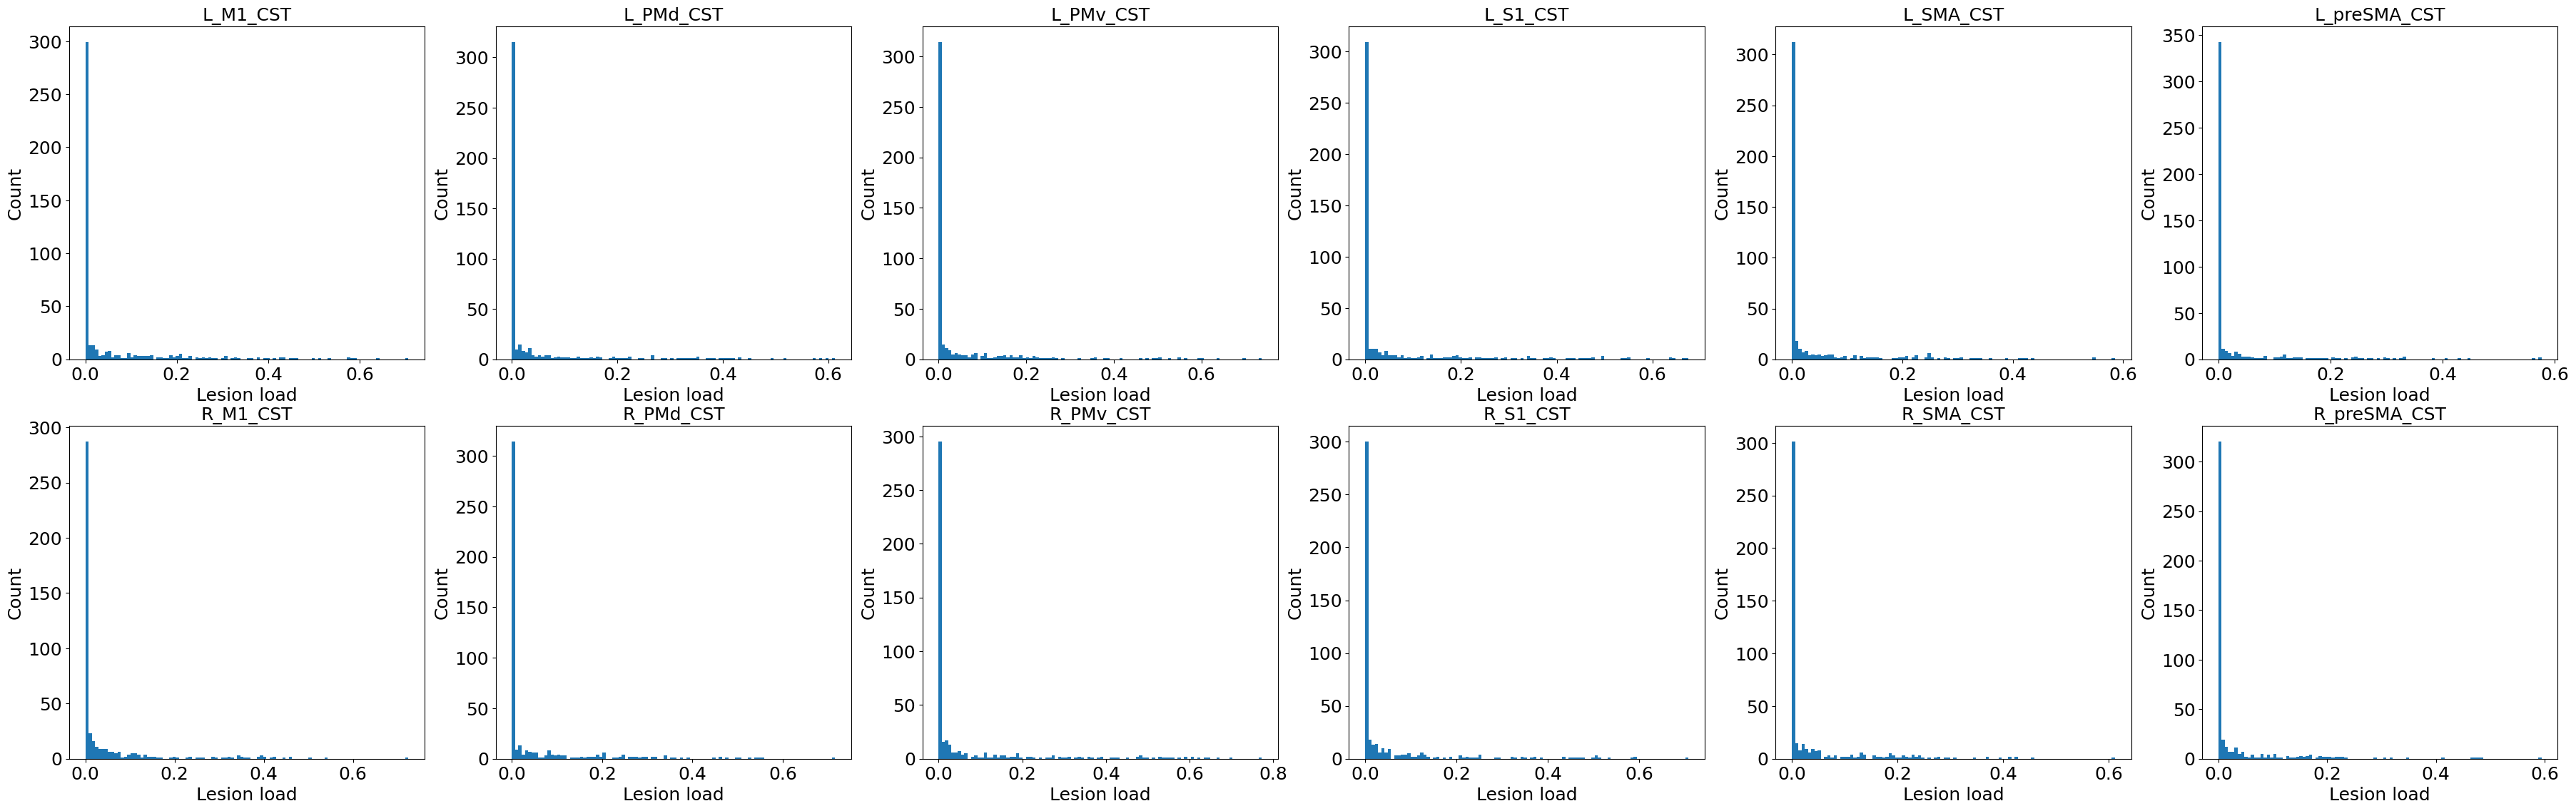
\includegraphics[width=1\linewidth]{figures/all2h_lesionload.png}
  \caption{Distributions of bihemispheric SMATT lesion load.}
  \label{fig:sfig2}
\end{subfigure}
\caption{Distribution of lesion load variables for chronic subjects.}
\label{lesion_load_dist}
\end{figure}


\begin{figure}[ht]
\centering
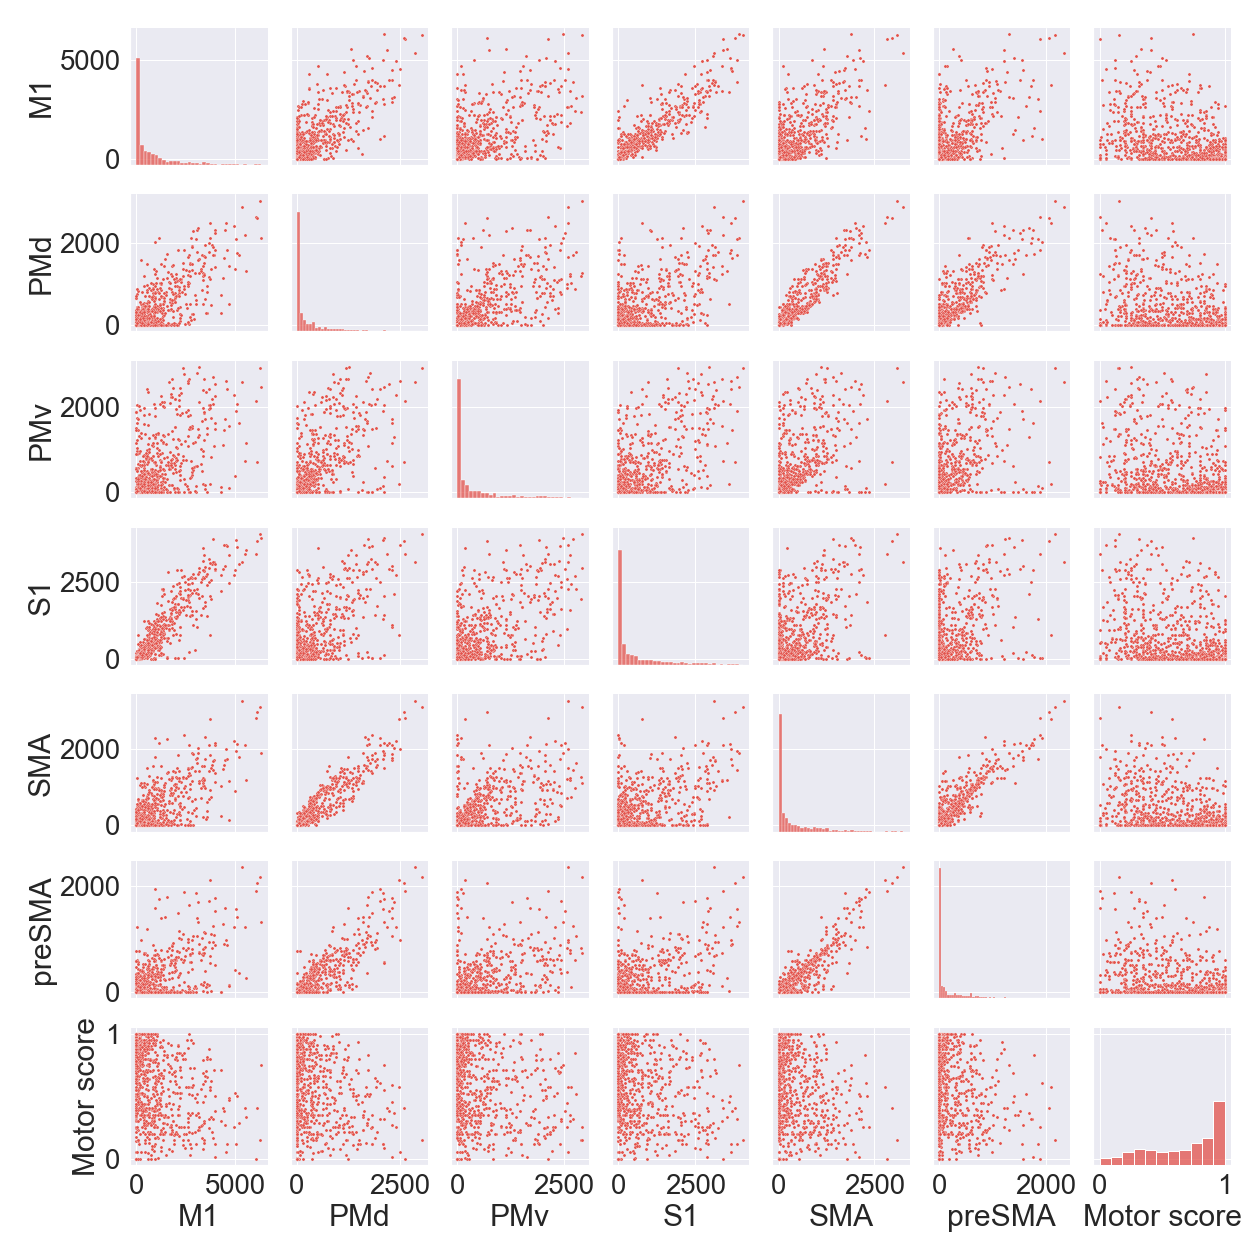
\includegraphics[width=0.8\linewidth]{figures/SMATT_scatterplts.png}
\caption{Correlations between lesion load calculated for each ipsilesional tract in the sensorimotor area tract template atlas.}
\label{smatt_pairwise_correlations}
\end{figure}


\begin{figure}[ht]
\centering
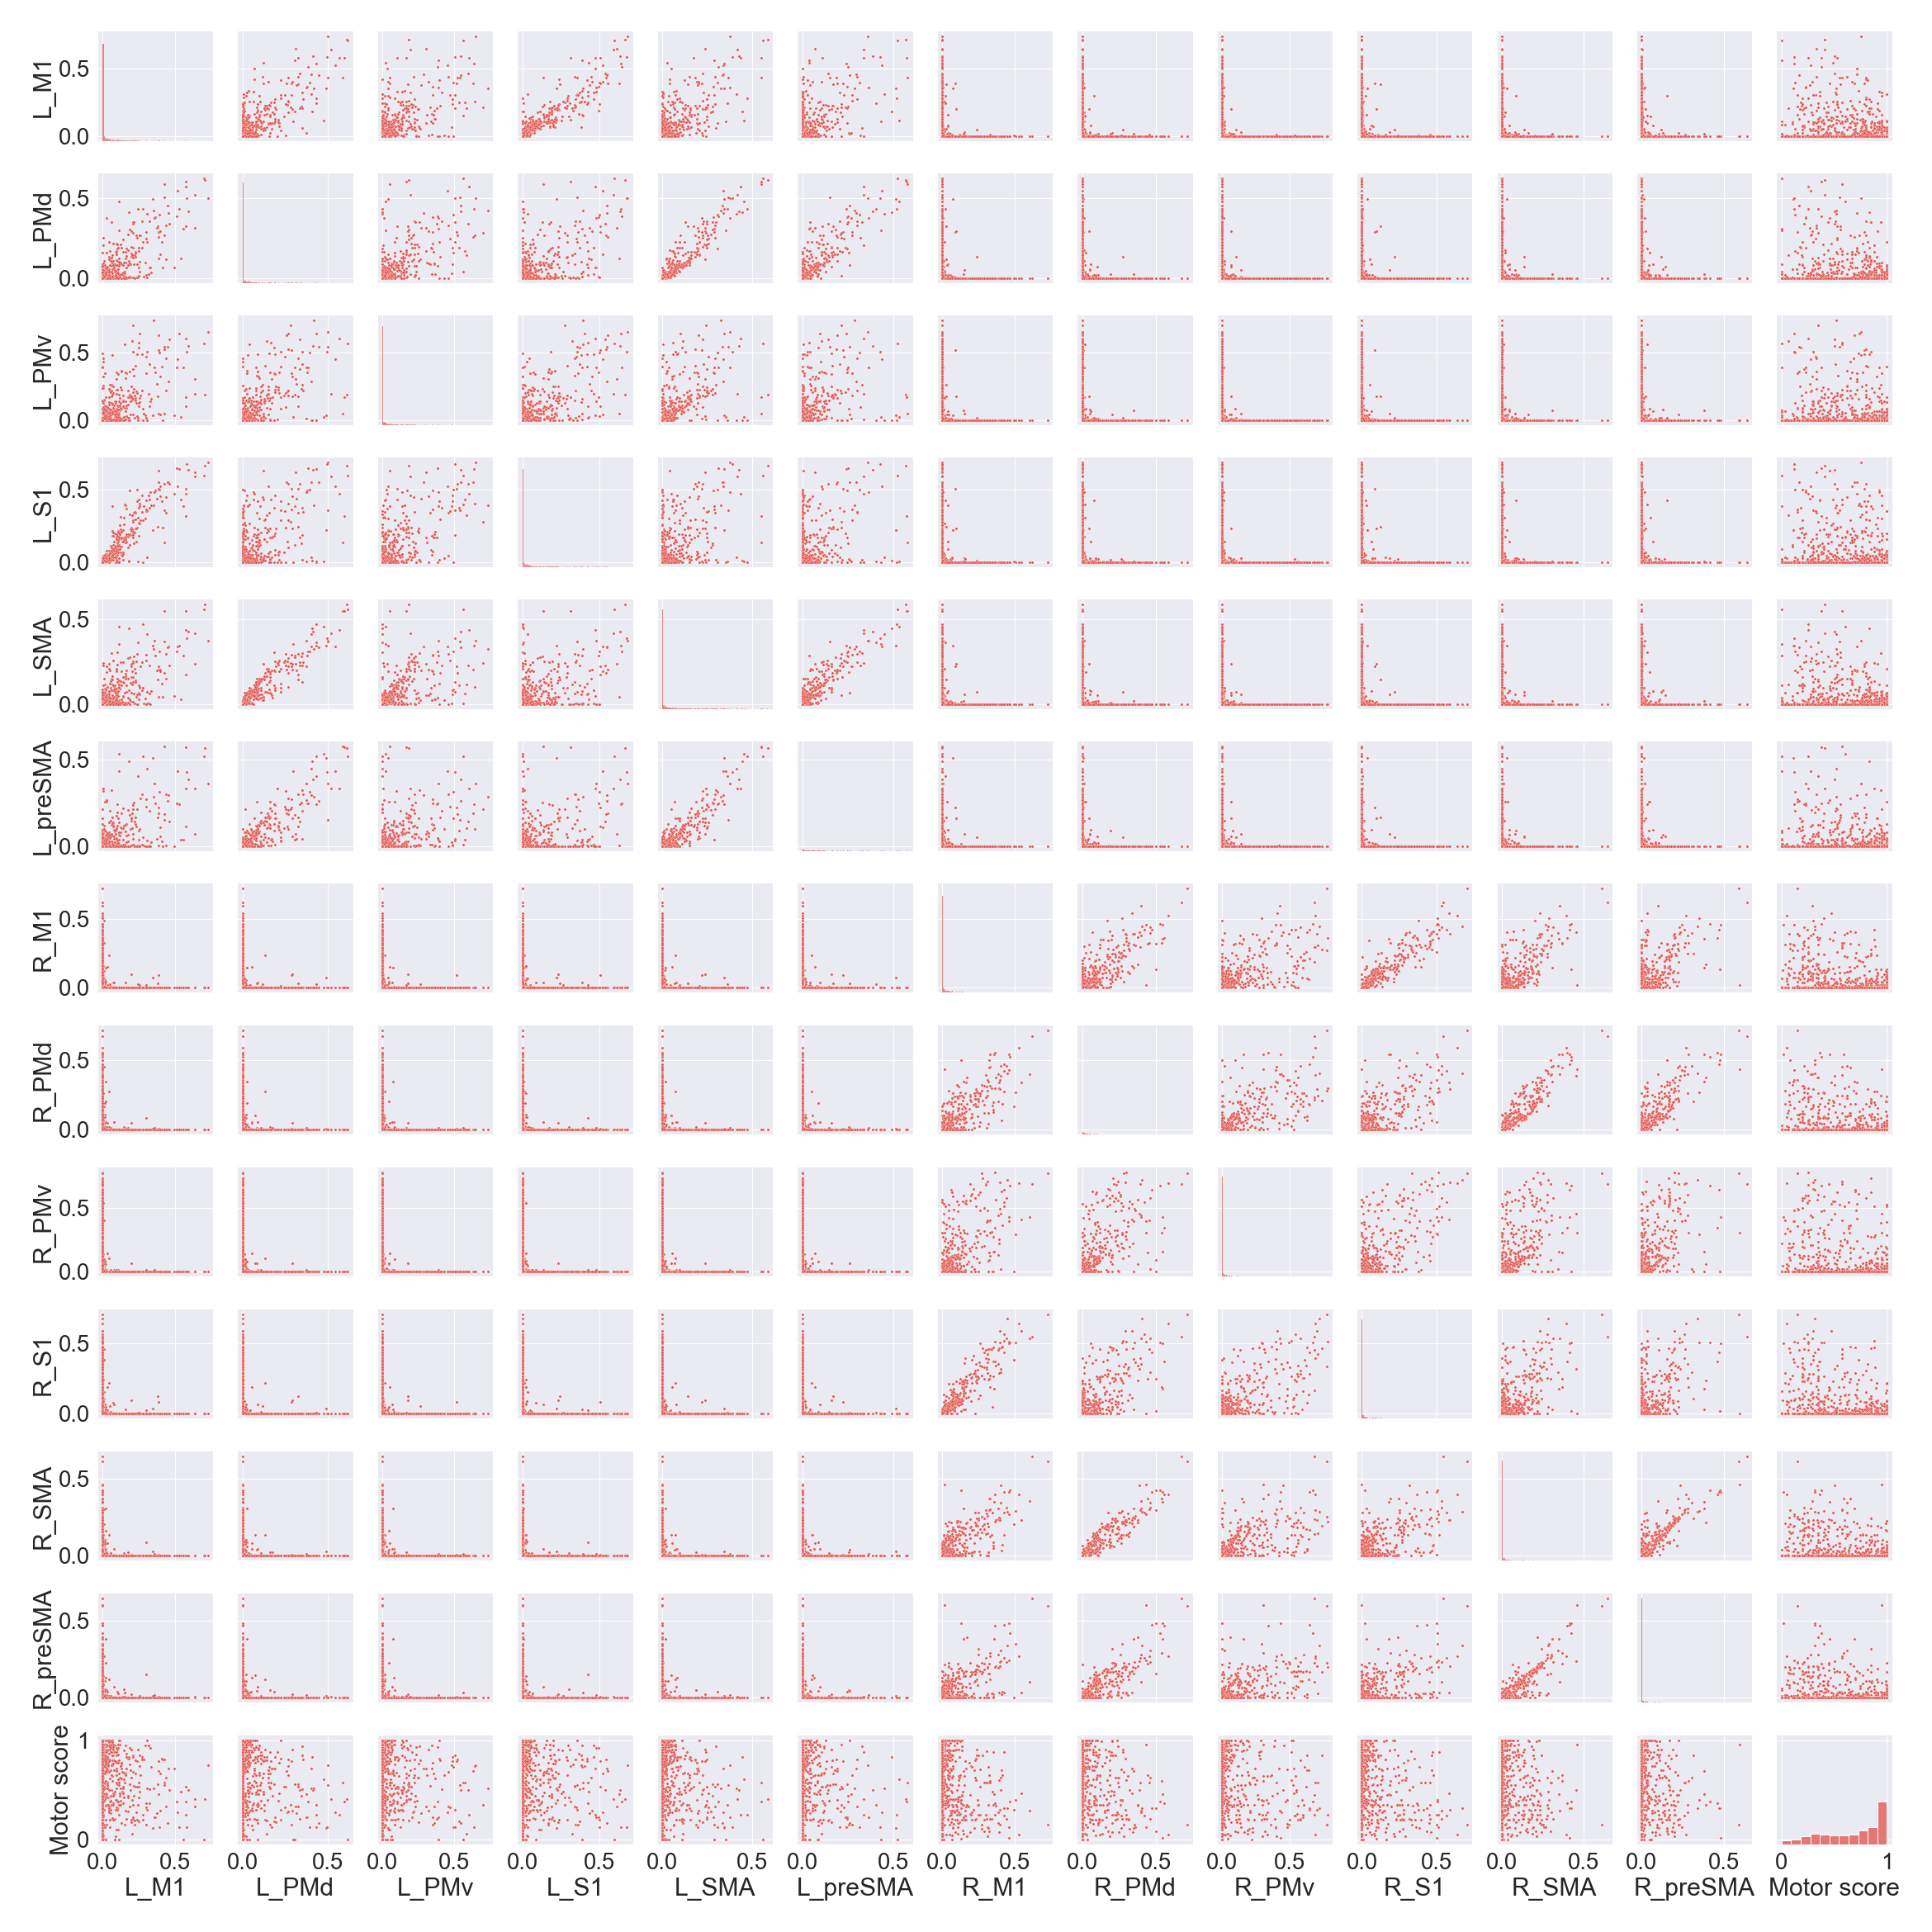
\includegraphics[width=1\linewidth]{figures/SMATT_bi_scatterplts.png}
\caption{Correlations between lesion load calculated for each tract in the sensorimotor area tract template atlas.}
\label{smatt_pairwise_correlations_bi}
\end{figure}




\begin{figure}[ht]
\centering
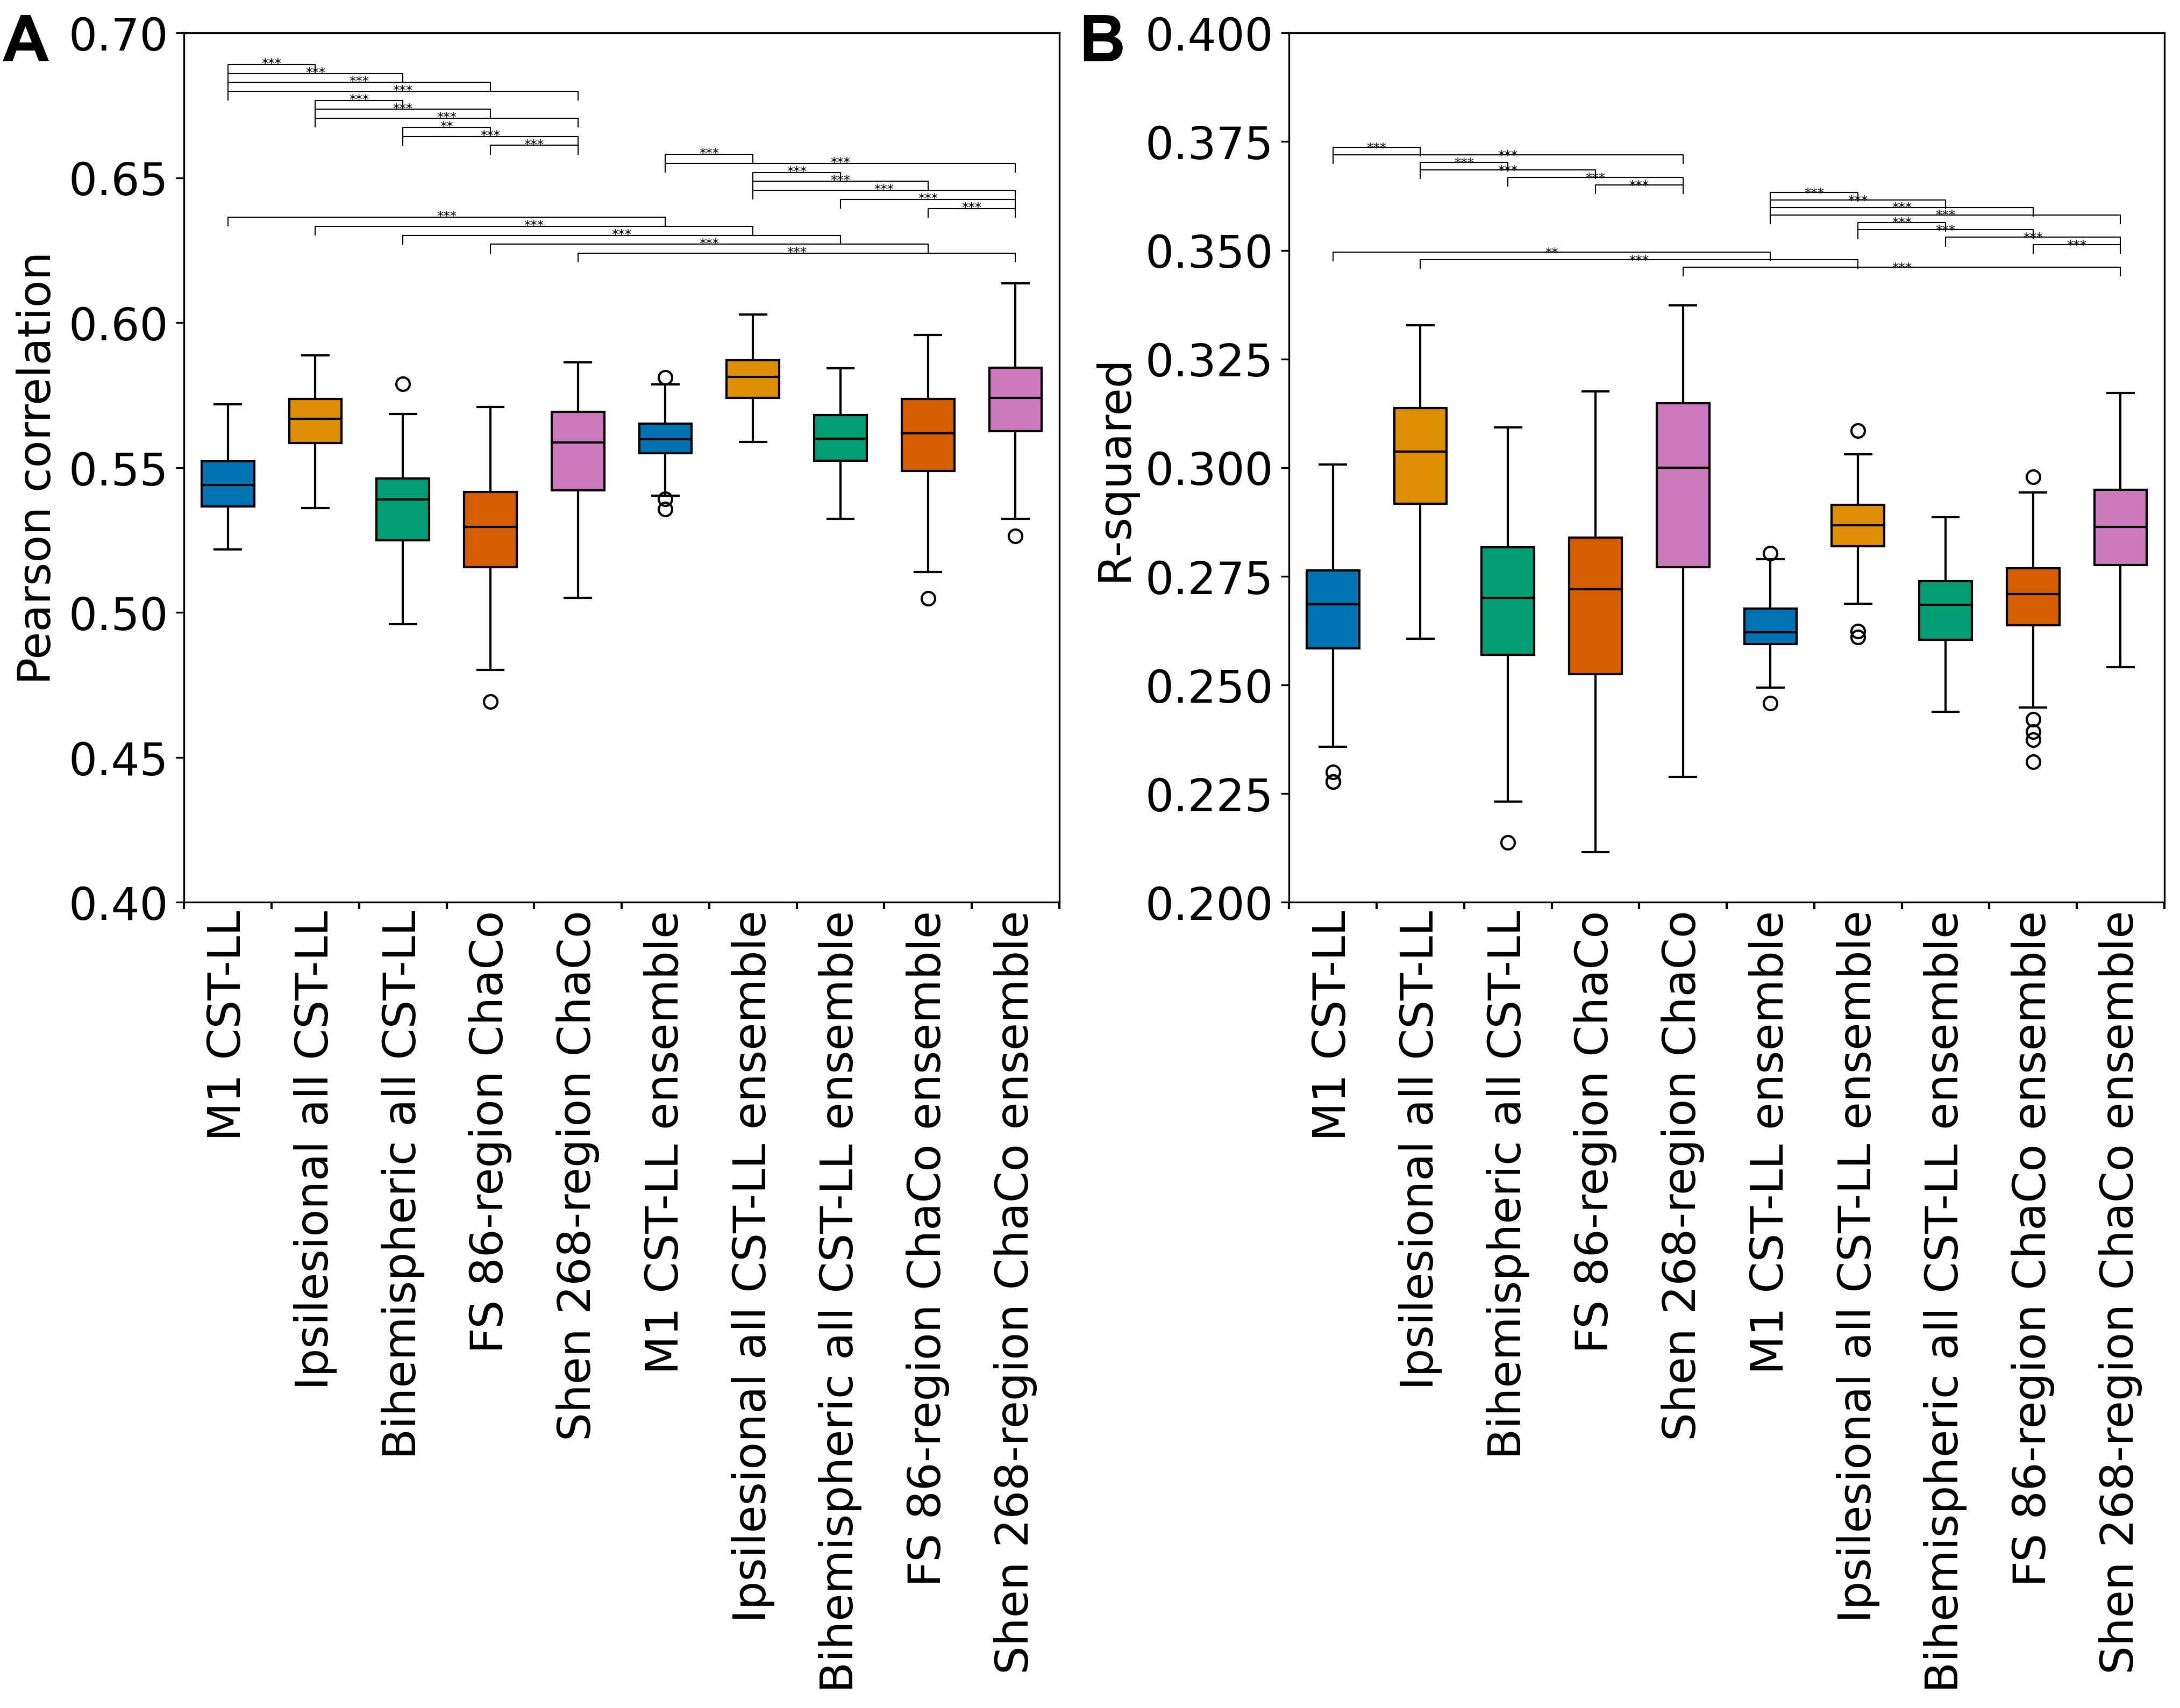
\includegraphics[width=1\linewidth]{figures/Analysis7.png}
\caption{Results from ensemble models with acute subjects (age, sex, time since stroke).}
\label{ensemble}
\end{figure}

\begin{table}[h]
\centering
\caption{Styled LaTeX Table}
\label{table:5}
\begin{tabular}{rrrrr}
\toprule
 &  & \multicolumn{2}{c}{Median performance} \\
 &  & Corr. (Std. dev.) & $R^2$ (Std. dev.) \\
\midrule
\multirow[t]{4}{*}{none} & M1 CST LL & 0.394 (0.004) & 0.142 (0.004) \\
 & Ipsi. SMATT LL & 0.430 (0.004) & 0.174 (0.004) \\
 & L/R SMATT LL & 0.446 (0.006) & 0.188 (0.006) \\
 & ChaCo (shen268) & 0.469 (0.010) & 0.210 (0.012) \\
\multirow[t]{4}{*}{demog} & M1 CST LL $\Plus$ demog. & 0.424 (0.005) & 0.173 (0.004) \\
 & Ipsi. SMATT LL $\Plus$ demog. & 0.457 (0.006) & 0.199 (0.004) \\
 & L/R SMATT LL $\Plus$ demog. & 0.462 (0.007) & 0.203 (0.004) \\
 & ChaCo (shen268) $\Plus$ demog. & 0.481 (0.009) & 0.215 (0.007) \\
\multirow[t]{6}{*}{chaco ll} & M1 CST LL $\Plus$ ChaCo (fs86) & 0.448 (0.005) & 0.199 (0.005) \\
 & Ipsi. SMATT LL $\Plus$ ChaCo (fs86) & 0.462 (0.006) & 0.212 (0.006) \\
 & L/R SMATT LL $\Plus$ ChaCo (fs86) & 0.469 (0.005) & 0.219 (0.005) \\
 & M1 CST LL $\Plus$ ChaCo (shen268) & 0.466 (0.005) & 0.216 (0.004) \\
 & Ipsi. SMATT LL $\Plus$ ChaCo (shen268) & 0.478 (0.006) & 0.226 (0.006) \\
 & L/R SMATT LL $\Plus$ ChaCo (shen268) & 0.482 (0.006) & 0.230 (0.006) \\
\multirow[t]{6}{*}{chaco ll demog} & M1 CST LL $\Plus$ ChaCo  (fs86) & 0.473 (0.006) & 0.212 (0.005) \\
 & Ipsi. SMATT LL $\Plus$ ChaCo  (fs86) & 0.489 (0.006) & 0.228 (0.005) \\
 & L/R SMATT LL $\Plus$ ChaCo  (fs86) & 0.491 (0.006) & 0.228 (0.005) \\
 & M1 CST LL $\Plus$ ChaCo  (shen268) & 0.483 (0.006) & 0.222 (0.005) \\
 & Ipsi. SMATT LL $\Plus$ ChaCo  (shen268) & 0.500 (0.007) & 0.237 (0.006) \\
 & L/R SMATT LL $\Plus$ ChaCo  (shen268) & 0.499 (0.007) & 0.237 (0.006) \\
\bottomrule
\end{tabular}
\end{table}

\begin{table}
\begin{tabular}{|l|l|r|r|r|r|}
%\captionof{table}{Site-specific demographic data.}
\hline {} &  Site &   N. &  N. F &  Mean age &  Mean normed motor \\ \hline
\textbf{0 } &  r001 &  39 &         10 &     59.62 &               0.62 \\ 
\textbf{1 } &  r002 &  12 &          6 &     65.75 &               0.45 \\
\textbf{2 } &  r003 &  15 &          6 &     59.53 &               0.26 \\ 
\textbf{3 } &  r004 &  19 &          7 &     44.63 &               0.20 \\ 
\textbf{4 } &  r005 &  27 &         12 &     64.93 &               0.67 \\
\textbf{5 } &  r009 &  57 &         16 &     67.84 &               0.92 \\ 
\textbf{6 } &  r010 &  26 &          7 &     57.15 &               0.97 \\ 
\textbf{7 } &  r011 &  28 &         10 &     57.21 &               0.89 \\ 
\textbf{8 } &  r015 &  15 &          0 &     59.60 &               0.72 \\ 
\textbf{9 } &  r017 &  14 &          0 &     57.43 &               0.52 \\
\textbf{10} &  r018 &  11 &          0 &     59.73 &               0.71 \\ 
\textbf{11} &  r021 &  12 &          0 &     60.83 &               0.90 \\
\textbf{12} &  r022 &  14 &          0 &     57.86 &               0.57 \\ 
\textbf{13} &  r023 &  14 &          8 &     58.00 &               0.43 \\ 
\textbf{14} &  r024 &  21 &          0 &     61.43 &               0.90 \\ 
\textbf{15} &  r025 &  16 &          3 &     64.19 &               0.73 \\ 
\textbf{16} &  r027 &  28 &          8 &     58.18 &               0.31 \\
\textbf{17} &  r028 &  21 &          6 &     58.14 &               0.74 \\
\textbf{18} &  r029 &   5 &          0 &     61.20 &               0.71 \\ 
\textbf{19} &  r031 &   1 &          0 &     52.00 &               0.68 \\ 
\textbf{20} &  r033 &   5 &          0 &     50.00 &               0.62 \\ 
\textbf{21} &  r034 &  15 &          6 &     57.26 &               0.80 \\ 
\textbf{22} &  r035 &  15 &          6 &     62.20 &               0.63 \\ 
\textbf{23} &  r038 &  18 &          7 &     62.17 &               0.88 \\ 
\textbf{24} &  r040 &  14 &          7 &     60.64 &               0.65 \\ 
\textbf{25} &  r042 &  22 &         11 &     50.55 &               0.61 \\ 
\textbf{26} &  r044 &   4 &          0 &     69.25 &               0.52 \\ 
\textbf{27} &  r045 &   4 &          1 &     59.75 &               0.48 \\ 
\textbf{28} &  r046 &  12 &          4 &     60.00 &               0.47 \\ 
\textbf{29} &  r047 &  44 &         14 &     64.84 &               0.62 \\
\textbf{30} &  r048 &  43 &         16 &     65.88 &               0.66 \\ 
\textbf{31} &  r052 &  32 &         12 &     61.09 &               0.41 \\ 
\textbf{32} &  r053 &   2 &          1 &     65.00 &               0.63 \\ 
\hline
\end{tabular}
\end{table}

The data shows the demographics and motor scores of subjects at different sites. Each row represents a site, and the columns show the site name, the number of subjects (N.), the number of female subjects (N. F), the mean age, and the mean normed motor score. The sites are numbered from 0 to 32. The number of subjects and the mean normed motor score vary across the sites, with some sites having more subjects and higher scores than others.

\end{document}